\documentclass{article}
\usepackage{graphicx}
\usepackage{mathtools} % loads amsmath \usepackage{amsmath}
\usepackage{amssymb}
\usepackage{eqnarray}
\usepackage{bm}

% Packages
\usepackage[utf8]{inputenc} % Required for inputting international characters
\usepackage[T1]{fontenc}    % Output font encoding for international characters
\usepackage[left=3cm, right=3cm, top=3cm,bottom=3cm]{geometry} 
\usepackage[english]{babel}
%\usepackage{amsmath}
\usepackage{caption}
\usepackage{amsmath}
\usepackage{graphicx}
\usepackage{epstopdf}
\usepackage{url}
\usepackage{times}  % Times font
\usepackage{setspace}
%\usepackage{datetime}
\usepackage{tocloft}
\usepackage{titlesec}
\usepackage{natbib}
\usepackage{fullpage}
\usepackage{physics}
\usepackage{amssymb}
\usepackage{ulem}
\usepackage{amsthm}
\usepackage[english]{babel}
\usepackage[title]{appendix}
\usepackage{pythonhighlight}
\usepackage[version=4]{mhchem}

\usepackage{listings}
\usepackage{xcolor}

\lstdefinelanguage{Julia}{
  morekeywords={
    function,end,if,else,elseif,for,while,return,struct,mutable,
    begin,let,where,using,import,module,export,const,local,
    global,true,false,nothing,try,catch,finally,do,in,break,
    continue
  },
  sensitive=true,
  morecomment=[l]\#,
  morestring=[b]",
}

\lstset{
  language=Julia,
  basicstyle=\ttfamily\small,
  keywordstyle=\color{blue},
  commentstyle=\color{green!50!black},
  stringstyle=\color{red},
  numbers=left,
  frame=single,
  breaklines=true,
  showstringspaces=false
}

\usepackage{hyperref}
\hypersetup{
    colorlinks,
    citecolor=black,
    filecolor=black,
    linkcolor=black,
    urlcolor=black
}


% my own dubble underscore
\def\dunder#1{\underline{\underline{#1}}}

\DeclareMathOperator\arctanh{arctanh}

\newtheorem{theorem}{Theorem}[section]
\newtheorem{corollary}{Corollary}[theorem]
\newtheorem{lemma}[theorem]{Lemma}
\newtheorem{definition}[theorem]{Definition}
\theoremstyle{remark}
\newtheorem{example}{Example}
\DeclareMathOperator{\sgn}{sgn}
\newcommand{\Log}{\text{Log}}

% Define new commands
\renewcommand{\cftsecfont}{\normalfont}
\renewcommand{\cftsecpagefont}{\normalfont}
\renewcommand{\cftsecleader}{\cftdotfill{\cftdotsep}}
\renewcommand{\cftsecaftersnum}{.}
\newcommand{\del}{\partial}
\titlelabel{\thetitle.\quad}


\newcommand{\minus}{\scalebox{0.75}[1.0]{$-$}}

\begin{document}
\begin{titlepage} 

	\begin{spacing}{2.0}
        \centering
	{\huge On methods of modelling the absorption and desorption of hydrogen in metal hydride materials using finite element methods and open source software
    }\\[.5cm] % Title of your document
	\end{spacing}
	
	\centering
	{\LARGE \doublespacing Tjipke Hofker - 4965558}\\
	\vspace{0.5cm}
	

    
	% \begin{figure*}[h]
    %     \centering
    %     \includegraphics[width=.4\linewidth]{figures/cover.png}
    %     \end{figure*}
        \vfill
\vspace{.5cm}	
 \begin{minipage}{0.49\textwidth}
		\begin{flushleft}
			MSC thesis\\
			TU Delft \\
            Applied Mathematics\\
            Delft, \today
		\end{flushleft}
	\end{minipage}
\hfill
	\begin{minipage}{0.49\textwidth}
		\begin{flushright}
			%Delft, \date{\today}\\
    {Supervisors:}  \makebox[4cm][l]{Dr. D.J.P. Domenico}\par
      \makebox[4cm][l]{Dr. J.L.A. Dubbeldam}\par
    	\end{flushright}
	\end{minipage}
		
\end{titlepage}
\newpage
{}
\pagebreak
\begin{titlepage}
    \textcolor{white}{a}
\end{titlepage}
\newpage
% page counting for abstract and toc I, II
\pagenumbering{roman}
\section*{Abstract}
The goal of this thesis is to implement a model for the absorption and desorption of hydrogen in metal hydride materials using finite element methods. The model will be implemented in Julia, and will be compared to a model implemented in Ansys Fluent by Rabienataj Darzi et al.\cite{RabienatajDarzi2016}. The model will be implemented in five different ways, starting with a 0D model of perfectly mixed absorption and desorption, then going to 1D and 2D models of absorption and desorption with pre-determined flow, and finally going to 1D and 2D models of absorption and desorption with flow calculated using the Navier-Stokes equations. The results of the models will be compared to each other.

\newpage
\vspace*{15mm}
\tableofcontents
\clearpage

% set page counting to arabic again (and 1)
\pagenumbering{arabic}
\setcounter{page}{1}

\section{Introduction}

When generating hydrogen gas from renewable energy sources, it is one of the cleanest forms of energy. The exhausted gases from burning hydrogen are only water ($H_2O$). It is therefore very promising to look at energy solutions based around hydrogen. A difficulty of hydrogen gas is transport. Since the gas is so light, it isn't energy dense. Traditionally, we use high-pressure gas cylinders or liquefied hydrogen storage, which require either extremely high pressures (up to 700 bar) or very low temperatures (around $-253$C), creating safety risks and high energy costs\cite{doe_hydrogen_storage}. A new and improving way is to use metal hydride materials. These materials give high gravimetric and volumetric density, high $H_2$ absorption capacity, moderate working temperature, and moderate charging pressure for $H_2$ storage. A solution to the heat generation and requirement when charging and discharging these batteries is the use of phase change materials. The implementation of these materials gives us the freedom to not use heaters or coolers in these batteries. The goal of this thesis is to model and experiment with different battery setups using metal hydride materials together with these phase change materials.

\subsection{Problem Introduction}

A lot of previous research has been done on the absorption and desorption of hydrogen in metal hydride materials for use as batteries or other methods of hydrogen storage \cite{Nemukula2025}. In addition, many numerical models have been developed to simulate these processes \cite{Sandrock1999}\cite{RabienatajDarzi2016}. The paper by Rabienataj Darzi et al.\cite{RabienatajDarzi2016} is the most relevant to this work, as it models the absorption and desorption of hydrogen in a metal hydride storage tank. Their model is implemented using the finite volume method in the commercial software Ansys Fluent \cite{Fluent}. Since the implementation is not publicly available and is based on finite volume methods, it cannot easily be reproduced, verified, or extended using finite element methods. The goal of this thesis is therefore to develop an open-source finite element implementation of the model and compare its results with those presented by Rabienataj Darzi et al.\cite{RabienatajDarzi2016}.

\subsection{Research Gap}

Although several numerical models for hydrogen absorption and desorption in metal hydride storage systems have been presented in the literature, most published implementations rely on commercial software or are not publicly available. As a result, there are few open-source finite element implementations that can be used to study these processes or serve as a basis for further research. This thesis addresses this gap by developing and validating an open-source finite element model for hydrogen absorption and desorption in a metal hydride storage tank.

\subsection{Research Question and Goal}

The main research question of this thesis is:

\begin{quote}
How can the absorption and desorption of hydrogen in metal hydride materials be modelled using finite element methods and only open-source software?
\end{quote}
To answer this question, the following subquestions are considered:

\begin{enumerate}
    \item How can we mathematically describe the physical processes governing the movement, absorption, and desorption of hydrogen in a metal hydride storage tank?
    \item How can the nonlinear absorption and desorption processes be incorporated into a finite element formulation?
    \item How can the governing equations be discretized in space using the finite element method?
    \item How can the resulting semi-discrete system be integrated efficiently and accurately in time?
\end{enumerate}

We aim to apply finite element methods to model the adsorption of $H_2$ gas in the battery. Finite element methods provide flexibility in handling complex geometries and heterogeneous materials, allow precise spatial resolution of physical processes, and are well-suited for solving coupled multiphysics problems. Combined with modern open-source scientific computing tools, this results in a flexible framework for exploring different battery configurations and evaluating their efficiency and response time.

The model will be implemented in Julia, a modern, high-performance programming language designed for technical and scientific computing. Julia combines ease of use with performance comparable to low-level languages and provides extensive support for scientific computing through open-source packages. In this work, Ferrite.jl is used for the finite element implementation, DifferentialEquations.jl for the time integration of the resulting systems, and MethodOfLines.jl to construct a finite difference implementation for validation of the finite element model.

% \subsection{Problem Introduction}

% A lot of previous research has been done on the absorption and desorption of hydrogen in metal hydride materials to use as batteries or other methods of hydrogen storage\cite{Nemukula2025}, and a lot of research has been done for modelling these processes\cite{Sandrock1999}\cite{RabienatajDarzi2016}. The last of which, the paper by Rabienataj Darzi et al.\cite{RabienatajDarzi2016}, is the most relevant to our work, as it looks at the absorption and desorption of hydrogen in metal hydride materials. This paper models using a finite volume implementation using the commercial software Ansys Fluent\cite{Fluent}. The model is not public, and uses finite volume methods. The goal of this thesis is to implement a model using finite element methods and open source software, and to compare the results of our model with the results of the model by Rabienataj Darzi et al.\cite{RabienatajDarzi2016}. 

% \subsection{Research Question and Goal}

% The goal of this thesis is to answer the question: How can we model the absorption and desorption of hydrogen in metal hydride materials using finite element methods using only open source software? 

% We aim to apply finite element methods to model the adsorption of $H_2$ gas in the battery. Finite element methods provide flexibility in handling complex geometries and heterogeneous materials, allow precise spatial resolution of physical processes, and are well-suited for solving coupled multiphysics problems. When combined, we hopefully end with a powerful tool to explore different battery configurations, and to evaluate their efficiency and response time.
% We will be modelling this in Julia, a modern, high-performance programming language designed for technical and scientific computing. Julia offers a combination of ease of use, speed comparable to low-level languages, and strong support for functional and mathematical programming paradigms. It is open source and has many libraries and packages for scientific computing, data analysis, and visualization. We will be using the DifferentialEquations.jl package for solving differential equations, the Ferrite.jl package for creating finite element problems, and the MethodOfLines.jl package for creating a finite difference approach to the problem to validate our results from the Finite Element Method.

\subsection{Report Contents}

We will be looking at five different models all increasing in complexity. The first model is a 0D model, where we assume the battery is perfectly mixed, and we will only look at the absorption and desorption of hydrogen in the metal hydride material. The second model is a 1D model, where we will look at the absorption and desorption of hydrogen in the metal hydride material, and we will assume flow of hydrogen is constant through the battery. The third model is a 2D model, where we will look at the absorption and desorption of hydrogen in the metal hydride material, and we will assume flow of hydrogen is constant through the battery. The fourth model will be a complete 1D implementation of the Navier-Stokes equations, where we will look at the absorption and desorption of hydrogen in the metal hydride material, and we model the velocity, density of the H2 gas, and the saturation of the metal hydride material. The fifth model will be a complete 2D implementation of our fourth model.

In Section~\ref{sec:physics} we will look at the physics behind the absorption and desorption of hydrogen in metal hydride materials, and the flow of hydrogen gas. In Section~\ref{sec:numerical_methods}, we will look at the numerical methods (Finite Difference Method, and the Finite Element Method), and we will discuss the time integration methods we will be using to solve our models. Lastly in this section, we look at the implementation of the numerical methods in Julia, and the packages we will be using to implement our models. In Section~\ref{sec:implementations} we will look at the different models we will be implementing, and how we will be implementing them. In Section~\ref{sec:results} we will look at the results of our models, and compare them to each other. In Section~\ref{sec:conclusion} we will conclude our findings, and look at future work that can be done in this area.

\vspace{.4cm}

This thesis is written as part of the Master of Applied Mathematics at the Technical University of Delft. The thesis is to be publicly defended on November the 27th, 2026. It is written by Tjipke Hofker, and supervised by Dr.~D.J.P. Domenico, and co-supervised by Dr.~J.L.A. Dubbeldam. The code can be found on GitHub\footnote{\url{https://github.com/ChocoTjip/MEP-tjipke-hofker}}.


% physics
\newpage
\section{Physics}\label{sec:physics}

In this section we will be looking at some of the physics behind the equations we will be using in our models. We start by looking at the absorption and desorption of Metal Hydride Materials in Section~\ref{subsec:metal_hydrides}, and explain how we get to the absorption equations in our models. Then we will be looking at the flow of our Hydrogen gas in Section~\ref{subsec:flow_model}, as these will be the most important equations for our models.

\subsection{Absorption and Desorption in Metal Hydride Materials}\label{subsec:metal_hydrides}

Metal Hydrides have been researched extensively. They are materials that can absorb Hydrogen gas, and store it in a solid form. This is done by the metal hydride absorbing the hydrogen gas, and forming a chemical bond with it. This is a reversible process, and the hydrogen can be released from the metal hydride by heating it up. This makes metal hydrides a good candidate for hydrogen storage, as they can store large amounts of hydrogen in a small volume. The chemical reaction for the absorption and desorption of hydrogen in metal hydrides is surprisingly simple, and can be given by the following chemical reaction\cite{Sandrock1999}:
\begin{align*}
    \ce{M + \frac{x}{2} H2 &<=>[\ce{H2}] MH_x}
\end{align*}
Where $M$ is the metal, $H_2$ is the hydrogen gas, and $MH_x$ is the metal with Hydrogen attached to it. $x$ is the number of hydrogen atoms that can be absorbed by the metal. The absorption and desorption of hydrogen in metal hydrides is a reversible, but has a hysteresis effect, meaning that the absorption and desorption curves are not the same. A schematic of the absorption and desorption curves can be seen in Figure~\ref{fig:absorption_desorption}. From now on if we talk about absorption,  we will be looking at the upper part of the curve, and if we talk about desorption, we will be looking at the lower part of the curve. For these parts, the mass absorption, and desorption rates are given by\cite{Jemni1995}:
\begin{align}
    \dot m(\rho, \rho_s) &= C_a \exp(- \frac{E_a}{R \, T}) \,
    \log( \frac{p_p}{p_{eq,a}} ) \, (\rho_{sat} - \rho_s(t)) \, ,\\
    \dot m(\rho, \rho_s) &= C_d \exp(- \frac{E_d}{R \, T}) \,
    (1 - \frac{p_p}{p_{eq,d}}) \, (\rho_s(t) - \rho_o) \, ,
\end{align}
where $C_a$ and $C_d$ are the absorption and desorption rate constants, $E_a$ and $E_d$ are the activation energies for absorption and desorption, $R$ is the universal gas constant, $T$ is the temperature, $p_p$ is the pressure of the hydrogen gas, $p_{eq,a}$ and $p_{eq,d}$ are the equilibrium pressures for absorption and desorption, $\rho_{sat}$ is the saturation density of the metal hydride, $\rho_s(t)$ is the density of the metal hydride at time t, and $\rho_o$ is the initial density of the metal hydride.

In both papers they also calculate the equilibrium pressures for absorption and desorption using the Van't Hoff equation, which is given by:
\begin{equation}
    \log\left(\frac{p_{eq}}{P_{ref}}\right) = A-\frac{B}{T}
\end{equation}
Where $P_{ref}$ is the reference pressure set to $1MPa$, $A$ and $B$ are constants that depend on the metal hydride, set to $10.7$ and $3704.6$ for absorption, and $10.57$ and $3704.6$ for desorption.

\subsubsection*{Model Assumptions}

In our first model we assume constant temperature, and pressure, and we will simplify the absorption and desorption rates accordingly. The gas is however not pure hydrogen, and $\rho_g$ will be the ratio of hydrogen in the gas mixture. The absorption and desorption rates will then be given by:

\begin{equation}\label{eq:phy_dotm_model1}
    \begin{aligned}
        \dot m(\rho_g, \rho_s) &= A_a^1 (\rho_{sat} - \rho_s(t)) \, \rho_g  \\
        \dot m(\rho_g, \rho_s) &= A_d^1 (\rho_s(t) - \rho_o) \, \rho_g 
    \end{aligned}
\end{equation}
where $A_a^1$ and $A_d^1$ are constants that depend on the temperature, pressure, and the properties of the metal hydride. In our more advanced models we will be modelling pressure and assume that the temperature is constant. Now $\rho_g$ is not a ratio of H2 gas in the mixture but the density of the purely H2 gas. We will then have the following absorption and desorption rates:
\begin{equation}\label{eq:dotm_model_4}
    \begin{aligned}
        \dot m(\rho_g, \rho_s) &= A_a^2 \log \left( \frac{RT\rho_g}{p_{eq,a}} \right)(\rho_{sat} - \rho_s(t))  \\
        \dot m(\rho_g, \rho_s) &= A_d^2 \left( 1 - \frac{RT\rho_g}{p_{eq,d}} \right)( \rho_s(t) - \rho_o) \, ,
    \end{aligned}
\end{equation}
where $A_a^2$ and $A_d^2$ are constants that depend on the temperature, and the properties of the metal hydride. We also assumed the ideal gas law to relate the pressure and density of the hydrogen gas.


\begin{figure}
    \centering
    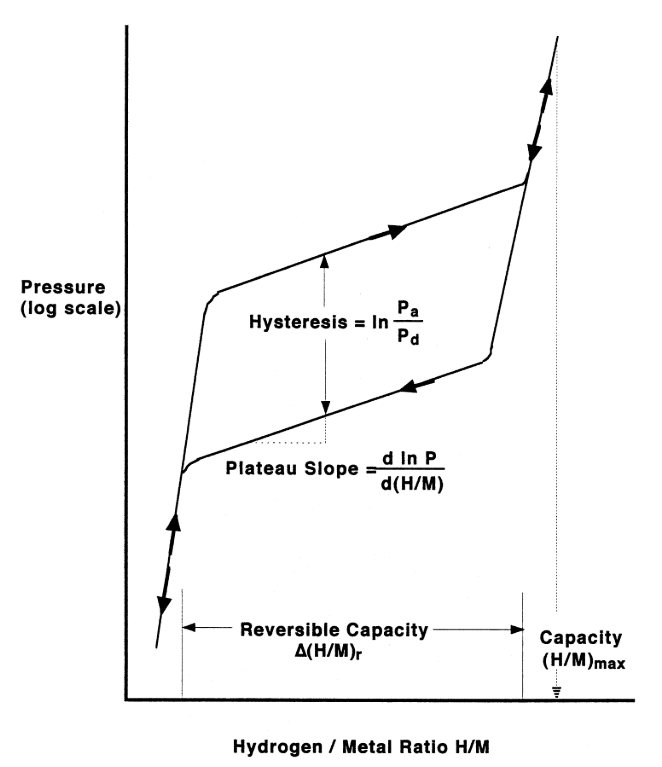
\includegraphics[width=0.4\textwidth]{figures/phy_hysteresis_curve.png}
    \caption{Schematic of the absorption and desorption curves of metal hydrides. The x-axis is the ratio between Hydrogen and Metal, and the capacity can therefor be interpreted as a measure for $x$ in $MH_x$. The absorption curve is the left and upper lines, the desorption is given in the right and lower lines. The hysteresis effect can be seen in the difference between the two curves. Schematic from Sandrock et al.\cite{Sandrock1999}}
    \label{fig:absorption_desorption}
\end{figure}


\subsection{Flow}\label{subsec:flow_model}
The governing equations consist of the conservation equations (mass, momentum and energy) together with constitutive equations describing the fluid properties. Assuming a Newtonian fluid, the constitutive relation for the stress tensor leads to the Navier–Stokes equations. The conservation equations are derived from the fundamental laws of physics, while the constitutive equations describe the material properties of the fluid. We will not be looking at the energy equation, as we assume constant temperature in our models. The conservation equations are given by (in their continuous form):

\begin{equation}\label{eq:continuity_equation}
    \partial_t \rho + \nabla \cdot (\rho \mathbf{u}) = \dot{m}
\end{equation}
Where $\rho$ is the density of the fluid, $\mathbf{u}$ is the velocity of the fluid, and $\dot{m}$ is the mass source term. The mass source term is given by the absorption and desorption rates we derived in Section~\ref{subsec:metal_hydrides}. The first term represents the local rate of change of mass, while the second term represents the net mass flux leaving the control volume. Together, they equal the volumetric mass source term due to absorption or desorption.

For Navier-Stokes, I like a little derivation starting from Newton's second law. Lets look at a small volume of fluid, now we get:

\begin{align*}
    \mathbf{F} &= m \, \mathbf{a} \\
    &= m \, \frac{D\mathbf{u}}{Dt} \\
    &= m \, (\partial_t \mathbf{u} + (\mathbf{u} \cdot \nabla) \mathbf{u}) \\
    \implies \frac{\mathbf{F}}{V} &= \rho \, (\partial_t \mathbf{u} + (\mathbf{u} \cdot \nabla) \mathbf{u})
\end{align*}
where $\mathbf{F}$ is the force, $m$ is the mass, $\mathbf{a}$ is the acceleration, $V$ is the volume, and $\rho$ is the density. Relevant forces acting on the fluid are the pressure gradient, the viscous forces, and we neglect any external forces (no gravity, no electromagnetic forces). These are given by:

\begin{align*}
    \frac{\mathbf{F}_{p}}{V} &= - \nabla p \\
    \frac{\mathbf{F}_{v}}{V} &= \mu \Delta \mathbf{u} \\
    % \frac{\mathbf{F}_{e}}{V} &= \mathbf{f}
\end{align*}
Where $p$ is the pressure, $\mu$ is the dynamic viscosity, and $\mathbf{f}$ is the external force. For the viscosity, we did assume a Newtonian fluid. Combining above equations, we get the Navier-Stokes equation:

\begin{align}
    \rho \, (\partial_t \mathbf{u} + (\mathbf{u} \cdot \nabla) \mathbf{u}) &= - \nabla p + \mu \Delta \mathbf{u}
\end{align}

Stokes:
\begin{equation}\label{eq:stokes_equation}
    \nabla \cdot \sigma + \mathbf{f} = 0
\end{equation}


\subsubsection*{Model Assumptions}
For our first spacially coupled models, we aim to measure the density of hydrogen gas $\rho_g$ in the battery, and the saturation of the metal hydride $\rho_s$. We do not yet aim to measure velocity of the gas and it is assumed that the flow is constant through the battery. The density of the hydrogen gas is seen as a fraction of the total density of the gas mixture, and we will assume that the gas mixture is incompressible. Thus in essence: $\rho = \rho_g + \rho_{other}$, where $\rho_{other}$ is the density of the other gases in the mixture. Since this is assumed constant, we can neglect it in our models, and we only have to look at Diffusion and Convection of the hydrogen gas:

\begin{equation}
    \left\{ \begin{aligned}
        \partial_t \rho_g &= D \nabla^2 \rho_g -\mathbf{v}\partial_x\rho_g - \dot{m}(\rho_g, \rho_s) \\
        \partial_t \rho_s &= \dot{m}(\rho_g, \rho_s)
    \end{aligned} \right.
\end{equation}
% \clearpage

\subsection*{Model Assumptions}

In this first model we do not yet look at the velocity, and pressure, and assume they are constant. The equations for the absorption of mass can then be given by:

\begin{align}
        \frac{D\rho_g}{Dt} &= -\dot{m}\label{eq:phy_drhogdt} \\
        \frac{D\rho_s}{Dt} &= \dot{m}\label{eq:phy_drhosdt}
\end{align}
where
\begin{equation}\label{eq:phy_stupidm}
    \dot{m} = A(\rho_{sat} - \rho_s(t)),
\end{equation}
with:
\begin{align}
    \rho_g(0) &= \rho_{g,0}, \\
    \rho_s(0) &= \rho_{s,0}.
\end{align}
If we look at Equation~\ref{eq:phy_drhosdt}, we can analytically solve:
\begin{align}
    \rho_s(t) &= \rho_{sat} - (\rho_{sat} - \rho_{s,0}) e^{-At} 
\end{align}
by looking at Equations~\ref{eq:phy_drhogdt} and~\ref{eq:phy_drhosdt}, we see that:
\begin{align}
    \frac{D\rho_g(t)}{Dt} &= -\frac{D\rho_s(t)}{Dt} \\
    \implies \rho_g(t) &= \rho_{g,0} - (\rho_s(t) - \rho_{s,0}) \\
    & = \rho_{g,0} + \rho_{s,0} - \rho_s(t) \\
    & = \rho_{g,0} + \rho_{s,0} - \rho_{sat} + (\rho_{sat} - \rho_{s,0}) e^{-At} 
\end{align}
say we move this to the 1D battery, then on the right hand side there initially is no hydrogen gas, and the metal hydride is not yet saturated. Now for this part we have (as long as no gas reaches here yet):
\begin{align}
    \rho_g(0) & = 0, \\
    \rho_s(0) & = 0, \\
    \rho_{sat} & = 1,
\end{align}
and after one second we have:
\begin{align}
    \rho_s(1) &= 1 - e^{-A} \\
    \rho_g(1) &= 0 + 0 - 1 + e^{-A} = e^{-A} - 1
\end{align}
giving a negative sign to our density of gas. This is because we do not take into account the density of gas in our mass transfer equations. While logically, there can only be mass transfer if there is gas. Since our density is a measure for the amount of hydrogen gas at that point, and our total gas density is constant, we can alter Equation~\ref{eq:phy_stupidm} to be:
\begin{equation}
    \dot{m} = A(\rho_{sat} - \rho_s(t))\frac{\rho_g(t)}{\rho_{g,total}},
\end{equation}
where $\rho_{g,total}$ is the total density of gas in the battery (which is constant). This way, if there is no hydrogen gas, there can be no mass transfer. 

% numerical methods
\newpage
\section{Numerical Methods}\label{sec:numerical_methods}

In this section we will be looking at the numerical methods used to solve the PDE's given in the previous section. 

A time-dependent partial differential equation is first discretized in space, resulting in a semi-discrete system of ordinary differential equations (or differential-algebraic equations). The spatial discretization may be performed using methods such as the Finite Difference Method, the Finite Volume Method, or the Finite Element Method. Subsequently, a time integration method is employed to obtain the fully discrete solution. This process is illustrated in Figure~\ref{fig:num_discretization_steps}. 

In the Sections~\ref{subseq:finite_element_methods}, and~\ref{subsec:finite_differences} we will be looking at the spacial discretization using Finite Element Methods, and Finite Differences respectively. They both tackle the problem of discretizing an equation in the following (continuous) form (with appropriate boundary and initial conditions):
\begin{equation}\label{eq:general_pde_numerical_methods}
    \mathcal{M}(u)\partial_t u = \mathcal{L}(u)+\mathcal{N}(u),
\end{equation}
where $u(x,t)$ is the variable we try to solve, $\mathcal{M}$ the weight or mass function, $\mathcal{L}$ a linear operator, and $\mathcal{N}$ a non-linear operator. The discretization of this equation leads to a semi-discrete system of ordinary differential equations (ODEs) or differential-algebraic equations (DAEs) of the form:
\begin{equation}\label{eq:semi_discrete_numerical_methods}
    M(\mathbf{u}) \frac{d\mathbf{u}}{dt} = L\mathbf{u}+N(\mathbf{u}),
\end{equation}
where $M(\mathbf{u})$ is a Mass Matrix, $\mathbf{u}$ is the spacially discretized control vector, with elements $u_i(t)$, $L$ is a linear operator matrix, and $N(\mathbf{u})$ is a non-linear operator vector. The interpretation of the discretized control vector is different depending on which spacial discretization method is used. In the case of Finite Differences, the control vector $\mathbf{u}$ contains the values of the function $u(x,t)$ at discrete points in space, while in the case of Finite Elements, the control vector $\mathbf{u}$ contains the coefficients of the basis functions used to approximate $u(x,t)$.

After the semi-discretization, we will be looking at the time integration methods used to solve the semi-discrete system of ODEs or DAEs. In Section~\ref{subseq:time_integrations} we will be looking at the different time integration methods used to solve the semi-discrete system of ODEs or DAEs. The time integration methods can be classified into two main categories: explicit and implicit methods. Explicit methods are generally easier to implement and computationally less expensive, but they may require smaller time steps for stability. Implicit methods are more stable and can handle larger time steps, but they require solving a system of equations at each time step, which can be computationally expensive. Initially, for the linear models we use a fully implicit method, while for the non-linear models we use a semi-implicit method. After this we go into more detailed methods for time integration, and state their advantages and disadvantages.

As we will see, both stages (spatial discretization and time integration) can cause stability issues. The stability of a spatial discretization method is often characterized by the Peclet number, which is a dimensionless number that characterizes the relative importance of convection and diffusion in a system. It is defined as:
\begin{equation}\label{eq:num_peclet}
    Pe = \frac{vh}{D},
\end{equation}
where $v$ is the characteristic velocity, $h$ is the characteristic length, and $D$ is the diffusion coefficient. The Peclet number can have a significant impact on the stability and accuracy of numerical methods, particularly for advection-dominated problems. In such cases, special techniques may be required to ensure stability and accuracy, such as upwinding or stabilization methods.

For time integration methods, the stability is often characterized by the Courant-Friedrichs-Lewy (CFL) number, also a dimensionless number that characterizes the stability of numerical methods for solving partial differential equations. It is defined as:
\begin{equation}\label{eq:num_cfl}
    CFL = \frac{v\Delta t}{h},
\end{equation}
where $v$ is the characteristic velocity, $\Delta t$ is the time step size, and $h$ is the spatial step size. The CFL condition states that for a numerical method to be stable, the CFL number must be less than or equal to a certain value, which depends on the specific method being used. If the CFL condition is violated, the numerical solution may become unstable and exhibit oscillations or blow up.

\begin{figure}
    \centering
    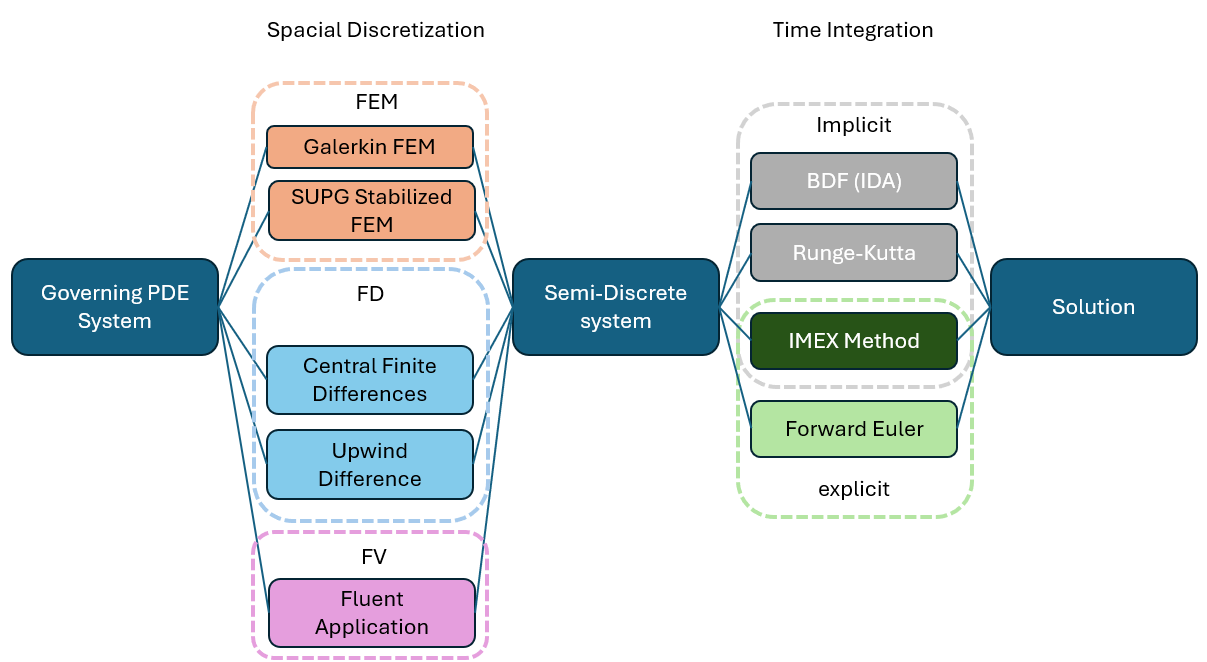
\includegraphics[width=\textwidth]{figures/Discretization_steps.png}
    \caption{The discretization steps to solve a PDE system. First we discretize in space, which we can do using Finite Differences, Finite Volumes, or Finite Elements. FD will be performed to check and validate solutions, and will be done using central finite differences, and Upwind methods. However this method quickly falls off and destabilizes for high Peclet numbers. We will create two types of FEM: the standard Galerkin method and the SUPG method for cases with a high Peclet number. Finite Volume is not looked at in this thesis, but is used in Darcy, and is very common in fluid models. Time integration is essentially independent from the spatial discretization, however often the best choice for time integration method is based on your choice of spatial discretization. These methods can be divided into Implicit and Explicit methods. We create our own IMEX method that combines both approaches. For our FEM with non-linear mass matrices, we will opt to use the IDA method, since we otherwise need to calculate an inverse or LU discretization at each time step. For a linear FEM with constant mass matrices, we use a fully implicit method. There are way more different discretization schemes, but these are the ones discussed in our thesis. It is also valuable to note that each spatial discretization is not unique; for example, you can often apply a Galerkin discretization on different spaces, giving different semi-discrete systems.}\label{fig:num_discretization_steps}
\end{figure}


\subsection{Finite Element Methods}\label{subseq:finite_element_methods}

In this subsection we will be looking at the discretization techniques Finite Element Methods entail, to tackle spatial discretization of functions of the form as seen in Equation~\ref{eq:general_pde_numerical_methods}. The core idea of a finite element method is to approximate the solution by a sum of finite element base functions, which are piecewise polynomial functions defined on a mesh of the domain. The finite element method then seeks to find the coefficients of these base functions that best approximate the solution to the PDE.

Say we have a PDE of the form:
\begin{equation}\label{eq:num_general_pde_numerical_methods}
    \partial_t\rho = -v\partial_x\rho \quad \text{in } \Omega
\end{equation}
where $\rho$ is the unknown function, $v$ is the flow speed, and $\Omega$ is the domain of interest. The finite element method aims to find the closest approximation of $\rho$ by a linear combination of finite element base functions $\psi^i$:
\begin{equation}
    \rho \approx \sum_i \rho^i \psi^i
\end{equation}
where $\rho^i$ are the coefficients to be determined. The finite element base functions $\psi^i$ are typically chosen to be piecewise polynomials that are defined on a mesh of the domain $\Omega$. The choice of the base functions and the mesh will depend on the specific problem and the desired accuracy of the solution. Now the way we will find the coefficients $\rho^i$ is by using test functions and testing whether they satisfy the PDE in a weak sense, so:

\begin{equation}
    \int_\Omega w^j \left( \partial_t\rho + v\partial_x\rho \right) dx = 0 \quad \forall j
\end{equation}
for a set of test functions $w^j$. In the Galerkin method, we choose the test functions to be the same as the finite element base functions, so $w^j = \psi^j$. 
\cite{toshniwal2024afe}

\subsubsection*{Lagrange Polynomials}
\subsection{Finite Differences}\label{subsec:finite_differences}

In this section we will be looking into finite difference methods. Finite difference methods are a class of numerical methods for solving differential equations by approximating derivatives with finite differences. The basic idea is to replace the continuous derivatives in the differential equation with discrete approximations based on the values of the function at a set of grid points. We use finite differences only as a check to validate our low-P\'eclet number FEM results, so we will not be looking very deeply into this method. We will describe finite differences with a simple example, show how this leads to oscilations, and then show how to fix this using upwind methods. 

A lot of the theory is implemented automatically in the MethodOfLines.jl package.

\subsubsection{Central Finite Differences}
Finite differences uses a discretization of the domain. Say we want to discretize the domain $[a, b]$ into $N$ intervals, we can define the discretization as follows:
\begin{equation}
    x_i = a + i\Delta x, \quad i = 0, 1, \ldots, N,
\end{equation}
where $\Delta x = (b-a)/N$ is the spatial step size. Now our control vector $\mathbf{u}$ becomes:
\begin{equation}
    \mathbf{u}(t) = \begin{pmatrix}
        u(x_0, t) \\
        u(x_1, t) \\
        \vdots \\
        u(x_{N-1}, t) \\
        u(x_N, t)
    \end{pmatrix}
\end{equation}

Say we have the simple diffusion equation:
\begin{equation}
    \partial_t u = D \partial_{xx} u,
\end{equation}
where $D$ is the diffusion coefficient. With initial condition and boundary conditions:
\begin{equation}
    \begin{aligned}
        u(x, 0) &= u_0(x), \\
        u(a, t) &= g_a(t), \\
        u(b, t) &= g_b(t),
    \end{aligned}
\end{equation}

Now we can approximate the second derivative using finite differences. The second derivative can be approximated using the central difference scheme:
\begin{equation}
    \partial_{xx} u(x_i, t) \approx \frac{u(x_{i+1}, t) - 2u(x_i, t) + u(x_{i-1}, t)}{\Delta x^2}.
\end{equation}
for all $i = 1, 2, \ldots, N-1$. This leads to a semi-discrete system of ODEs:
\begin{equation}
    \partial_t \mathbf{u}(t) = D A \mathbf{u}(t),
\end{equation}
where $A$ is the matrix representing the finite difference approximation of the second derivative. The matrix $A$ is a tridiagonal matrix with the following structure:
\begin{equation}
    A = \frac{1}{\Delta x^2} \begin{pmatrix}
        -2 & 1 & 0 & \cdots & 0 \\
        1 & -2 & 1 & \cdots & 0 \\
        0 & 1 & -2 & \cdots & 0 \\
        \vdots & \vdots & \vdots & \ddots & 1 \\
        0 & 0 & 0 & 1 & -2
    \end{pmatrix}.
\end{equation}
for the boundary points corresponding to $i = 0, N$ we can use Dirichlet boundary conditions, where we set the values of $u(x_0, t)$ and $u(x_{N}, t)$ to be constant. This leads to a semi-discrete system of ODEs that can be solved using time integration methods as discussed in Section~\ref{subseq:time_integrations}.

\subsubsection{Upwind Methods}

The above method often leads to numerical oscillations in the solutions if we are working with advective problems. These are due to the use of central differences at the boundaries and discontinuities in the solution. If you take for example a simple advection equation:

\begin{equation*}
    \partial_t u + c \partial_x u = 0,
\end{equation*}
where $c$ is a constant, and $u(x,t)$ is the solution we are approximating. The solution is of the form:

\begin{equation*}
    u(x,t) = f(x - ct)
\end{equation*}
and represents a wave moving to the right with speed $c$ (assuming $c$ is positive). Take above equation for example, and apply central differences to a step:
\begin{equation*}
    \partial_x u_n \approx \frac{u_{n+1} - u_{n-1}}{2h},
\end{equation*}
If you apply this to a vector $\mathbf{u}$ with a steep gradient/discontinuity, we get the following result for the derivative with respect to $x$:
\begin{equation*}
    \mathbf{u}^i = \begin{pmatrix}
        \vdots \\ 1 \\ 1 \\ 1 \\ 0 \\ 0 \\ 0 \\ \vdots
    \end{pmatrix}, \qquad \implies \qquad
    \partial_x \mathbf{u}^i \approx \begin{pmatrix}
        \vdots \\ 0 \\ 0 \\ -\frac{1}{2h} \\ -\frac{1}{2h} \\ 0 \\ 0 \\ \vdots
    \end{pmatrix}
\end{equation*}
and since the change wrt time is given by $\partial_t \mathbf{u}^i = -c \partial_x \mathbf{u}^i$, we get the following result for the time derivative:
\begin{equation*}
    \partial_t \mathbf{u}^i \approx \begin{pmatrix}
        \vdots \\ 0 \\ 0 \\ \frac{c}{2h} \\ \frac{c}{2h} \\ 0 \\ 0 \\ \vdots
    \end{pmatrix}
\end{equation*}
The value immediately upstream of the discontinuity increases above its physical value, while the downstream value also begins to increase. After repeated time integration these non-physical updates propagate through the domain and develop into the oscillatory behaviour observed in central difference discretizations of advection-dominated problems. This is not what we want, and leads to numerical oscillations in the solution; The central difference scheme uses information from both sides of the point, instead of only upstream (which should be the case for a moving wave). Also, it is not taking into account the value of $u_n$ itself. 

The upwind method checks the direction of the flow and uses information from the upstream side to compute the solution at a given point. This method is particularly useful for problems involving advection or convection, where the direction of the flow is important. The upwind method can help to reduce numerical oscillations and improve stability in the solution. Implementing above example using the upwind method, if we have a positive flow velocity, we will get a forward difference scheme:
\begin{equation*}
    \partial_x u_n \approx \frac{u_{n} - u_{n-1}}{h},
\end{equation*}
which, in the example above, gives us the following result for the derivative with respect to $x$:
\begin{equation*}
    \partial_x \mathbf{u}^i \approx \begin{pmatrix}
        \vdots \\ 0 \\ 0 \\ 0 \\ -\frac{1}{h} \\ 0 \\ 0 \\  \vdots
    \end{pmatrix},
\end{equation*}
and now the change wrt time is given by:
\begin{equation*}
    \partial_t \mathbf{u}^i = -c \partial_x \mathbf{u}^i \approx \begin{pmatrix}
        \vdots \\ 0 \\ 0 \\ 0 \\ \frac{c}{h} \\ 0 \\ 0 \\ \vdots
    \end{pmatrix},
\end{equation*}
which will lead to a growth of only the part upwind of the continuity, as expected. The method above is seen as the first order upwind method. To reduce numerical diffusion, we can use a second order upwind method, which uses a second order approximation of the derivative[SOURCE]:
\begin{equation*}
    \partial_x u_n \approx \frac{3u_n - 4u_{n-1} + u_{n-2}}{2h},
\end{equation*}
this leads to a more accurate approximation of the derivative, and reduces numerical diffusion, but is more computationally expensive.

The ideas behind the upwind method is shown in Figure~\ref{fig:num_upwind}. Here we see the appriximations for the derivative at a certain point given the direction of the flow. 
\begin{figure}
    \centering
    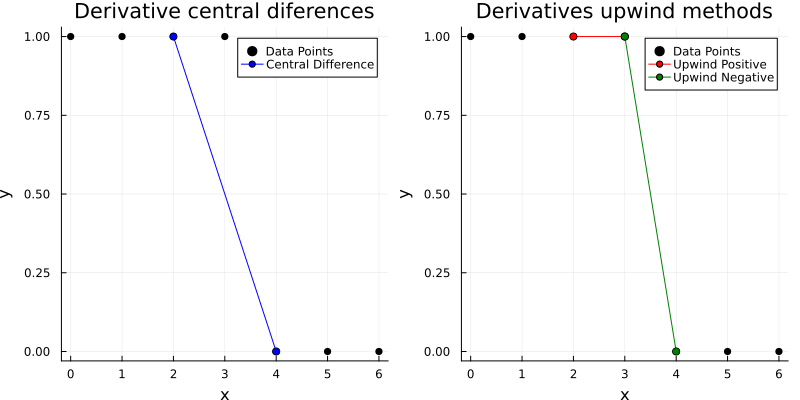
\includegraphics[width=\textwidth]{figures/num_upwind.png}
    \caption{The left figure shows the derivative at point $x=3$ for the central differences method, and the right figure shows the results of the upwind method. The central differences will give a wrong picture if the velocity is positive (moving to the right), because of how the derivative is calculated. For the upwind method we look at different derivatives depending on the direction of the flow. If the flow is positive, we use the red derivative, and if the flow is negative, we use the green derivative.}\label{fig:num_upwind}
\end{figure}

% vind volgende stukken nog leuk maar niet af en dus niet zeker of ik ze wil houden
% Fourier analysis/stability and fourier analysis

% \subsubsection*{stability}
% Another way of seeing the osscilations happen in the central difference scheme is by looking at the effect it has on fourier series. Since we know every smooth enough function is approximable by a fourier series, we can look at the effect of the central difference scheme on a fourier series. Take for example the following fourier series:
% \begin{equation*}
%     u(x) = \sum_{k=-\infty}^{\infty} \hat{u}_k e^{ikx},
% \end{equation*}
% where $\hat{u}_k$ are the fourier coefficients. Now we can look at the effect of the central difference scheme on this fourier series:
\subsection{Time Integration}\label{subseq:time_integrations}

In the previous section, the governing partial differential equations were spatially discretized. This transformed Equation~\ref{eq:general_pde_numerical_methods} into the semi-discrete system given by Equation~\ref{eq:semi_discrete_numerical_methods}. The spatial dependence is therefore represented by a finite number of degrees of freedom, while time remains continuous. The purpose of time integration is to transform this semi-discrete system into a system that can be solved at discrete points in time. That is what we will be tackling in this section. A few methods that we later apply will be described here.

The simplest time integration methods are the forward and backward Euler methods. The forward Euler method is an explicit method, while the backward Euler method is an implicit method. Implicit is more accurate but computationally more expensive for non-linear problems, as it requires solving a system of equations at each time step. Explicit is easier to compute but less accurate, and requires smaller time steps for stability. Initially I wrote a combined method that uses implicit for linear terms and explicit for non-linear terms. This is an IMEX method, which we will describe in Section~\ref{subsubsec:num_IMEX}.

For our methods where the time-dependency is written in the form $Md\mathbf{u}/dt = \mathbf{f}(\mathbf{u},t)$, we can use the builtin Julia \texttt{Rodas5P} function. This method is an implicit fifth-order Rosenbrock--Wanner method, which we will briefly describe in Section~\ref{subsubsec:num_ROW}.

For our models with a time dependent mass matrix, say if it depends on the density at that $x$, we cannot easily write it in the system that is compatible with \texttt{Rodas5P}. In this case, we can use the \texttt{IDA} function from the \texttt{Sundials.jl} package. This method is a variable-step, variable-order backward differentiation formula method, which is designed for fully implicit differential-algebraic systems.

Lastly, the time-integration method used together with \texttt{MethodOfLines.jl} is discussed. This package is used to obtain finite-difference reference solutions for Models~4 and~5 at sufficiently low P\'eclet numbers. After the spatial discretization has been generated, the resulting system is integrated using the \texttt{Tsit5} method. The Tsitouras method is an explicit fifth-order Runge--Kutta method with an embedded fourth-order error estimator. The embedded estimator allows the local temporal error to be estimated and the time-step size to be adjusted automatically. Since it is an explicit method intended primarily for non-stiff systems, it is used here for the validation cases in which the semi-discrete equations can be integrated efficiently without requiring a stiff solver.

\subsubsection{Implicit--Explicit (IMEX) Method}\label{subsubsec:num_IMEX}

Implicit methods are generally more accurate than explicit methods, but for non-linear problems they require solving a system of equations at each time step, which can be computationally expensive. The most famous example of an implicit method of a system is the backward Euler method. Given a system of ordinary differential equations in the form $M \dot{\mathbf{u}} = \mathbf{f}(\mathbf{u},t)$ (with $\dot{\mathbf{u}}=du/dt$), we apply backwards integration:

\begin{equation}
    \frac{M\mathbf{u}^{n+1} - M\mathbf{u}^n}{\Delta t}= \mathbf{f}(\mathbf{u}^{n+1},t^{n+1}),
\end{equation}
Which we can rewrite as:

\begin{equation}
M\mathbf{u}^{n+1} = M\mathbf{u}^{n} + \Delta t \mathbf{f}(\mathbf{u}^{n+1},t^{n+1}),
\end{equation}
where $\mathbf{u}^{n}$ is the solution at time $t^{n}$, $\Delta t$ is the time step size. The backward Euler method is unconditionally stable, but it can be computationally expensive for non-linear problems because it requires solving a system of equations at each time step. If $f$ is linear, the system becomes the simple:
\begin{equation}
(M-\Delta t A)\mathbf{u}^{n+1} = M\mathbf{u}^{n},
\end{equation}
where $A$ is the matrix representation of the linear operator. This can be solved directly by calculating $\mathbf{u^{n+1}}=(M-\Delta t A)^{-1}M\mathbf{u}^{n}$. But if $f$ is non-linear, we need to use an iterative method such as Newton's method to solve for $\mathbf{u}^{n+1}$, so the implicit method requires more work. 

The most famous example of an explicit method is the forward Euler method. Given a system of ordinary differential equations in the form $M\dot{\mathbf{u}} = \mathbf{f}(\mathbf{u},t)$, we apply forward integration:

\begin{equation}
    \frac{M\mathbf{u}^{n+1} - M\mathbf{u}^n}{\Delta t}= \mathbf{f}(\mathbf{u}^{n},t^{n}),
\end{equation}
Which we can rewrite as:
\begin{equation}
M\mathbf{u}^{n+1} = M\mathbf{u}^{n} + \Delta t \mathbf{f}(\mathbf{u}^{n},t^{n}),
\end{equation}
The forward Euler method is conditionally stable, which means that it requires a sufficiently small time step size to be stable. The stability condition is given by the Courant--Friedrichs--Lewy (CFL) condition, which states that the time step size must be less than or equal to the spatial grid size divided by the maximum wave speed in the system. The IMEX method combines the best of both worlds by using an implicit method for the linear terms and an explicit method for the non-linear terms. This allows for larger time steps while still maintaining some stability and accuracy. For a problem written as:
\begin{equation}
M\dot{\mathbf{u}} = A\mathbf{u} + \mathbf{f}(\mathbf{u},t),
\end{equation}
the IMEX method becomes:
\begin{equation}
(M-\Delta t A)\mathbf{u}^{n+1} = M\mathbf{u}^{n} + \Delta t \mathbf{f}(\mathbf{u}^{n},t^{n}),
\end{equation}
which is again easily solvable. This method especially worked well in model 2 and 3, where a large part of the physics that typically cause stiffness or instability are linear, and the non-linear terms are less stiff (the absorption and desorption of the hydrogen gas).

\subsubsection{Linear-Implicit Newton}

In the previous section we looked at how we can construct an implicit method from linear terms, and an explicit method from non-linear terms. If the problem has non-linear terms that form unstable integrations using explicit methods, we need to look at how to solve this implicitly as well. The backwards Euler method is (for what I can tell), the cornerstone of these implicit solvers, and many other such methods are alterations during the linear solve step or time step but follow the same principles (like the ROW method that we will be looking at in the next section). That is why I dedicate a section to this solver (even if we do not directly use it).

As per our previous example we have a discretization of the form:

\begin{equation}\label{eq:num_linear-implicit-newton_Mdotu}
    M\dot {\mathbf{u}} = \mathbf{f}(\mathbf{u},t)
\end{equation}

when using backward euler we evaluate all $u$ terms at the next time step. Leading to the a `residual equation' of the form:
\begin{equation}\label{eq:num_res_implicit_euler}
    \mathbf{R}(\mathbf{u}^{n+1}) = M(\mathbf{u}^{n+1} - \mathbf{u}^{n}) - \Delta t \mathbf{f}(\mathbf{u}^{n+1},t^{n+1}) = 0
\end{equation}
which is a non-linear system of equations. To solve this we use Newtons method. This is an iterative method for finding $u^{n+1}$ such that the residual is (very close to) zero. We start with an initial guess for $u^{n+1}$, which we call $u^{n+1}_0$. Say, $u^{n+1}_0 = u^n$.  This gives us a residual $R(u^{n+1}_0)$. We then linearize the residual around this guess, and solve for a correction $\delta u$ such that:
\begin{equation}
    \mathbf{R}(\mathbf{u}^{n+1}_0 + \delta \mathbf{u}) \approx \mathbf{R}(\mathbf{u}^{n+1}_0) + J_R(\mathbf{u}^{n+1}_0) \delta \mathbf{u} = 0
\end{equation}
where $J_R$ is the Jacobian of the residual with respect to $u^{n+1}$. This gives us a linear system of equations to solve for $\delta u$:
\begin{equation}
    J_R(\mathbf{u}^{n+1}_0) \delta \mathbf{u} = -\mathbf{R}(\mathbf{u}^{n+1}_0)
\end{equation}
We then update our guess:
\begin{equation}\label{eq:num_step_update_implicit_euler}
    \mathbf{u}^{n+1}_1 = \mathbf{u}^{n+1}_0 + \delta \mathbf{u}
\end{equation}
and repeat the process until convergence. If we know the Jacobian of $f$ with respect to $u$, $J_f$, we can compute the Jacobian of the residual, Equation~\ref{eq:num_res_implicit_euler}, as:
\begin{equation}\label{eq:num_jacobian_residual_implicit_euler}
    J_R(\mathbf{u}^{n+1}) = M - \Delta t J_f(\mathbf{u}^{n+1},t^{n+1})
\end{equation}
and we can rewrite Equation~\ref{eq:num_step_update_implicit_euler} as:
\begin{equation}
    \mathbf{u}^{n+1}_1 = \mathbf{u}^{n+1}_0 - J_R(\mathbf{u}^{n+1}_0)^{-1} \mathbf{R}(\mathbf{u}^{n+1}_0)
\end{equation}
now we repeat until the residual is sufficiently small, or it is sufficiently small wrt the solution. One more important note is that the time step $\Delta t$ in Equation~\ref{eq:num_jacobian_residual_implicit_euler} is often written in literature (especially literature for Julia) as $\gamma$. And the jacobian of the residual is $W$. Giving:
\begin{equation}
    W = M-\gamma J_f
\end{equation}

\subsubsection{Rosenbrock--Wanner (ROW) method}\label{subsubsec:num_ROW}

In the previous section we looked at implicit time integration for non-linear terms using backward Euler. 

\subsubsection{Implicit Differential-Algebraic (IDA) Methods}\label{subsubsec:num_IDA}

In our applications of Navier-Stokes, we have $\rho \dot{\mathbf{v}}$ at the left hand side as the momentum term, which gives us a density-dependent mass matrix. Since the control vector contains both $\rho$, and $\mathbf{v}$, we end up with a left hand side of the form $M(\mathbf{u})\dot{\mathbf{u}}$. The main issue with going about this problem in the same way as the previous sections, is that it requires a linear solve involving the state-dependent $M$ every time the RHS is evaluated, and it fails as an explicit reformulation if $M$ is singular. A method that would not need this extra linear solve are methods that look at a DAE (set of Differential Algebraic Equation). This can be viewed as a generalized backward Euler method, where we do not seperate partial derivatives wrt time to the lhs, and the rest to the rhs. It gives a very powerfull tool to solve any combination of differential and algebraic equations. In this section we will explain the mathematics stated in the sundials website\footnote{\url{https://sundials.readthedocs.io/en/latest/ida/Mathematics_link.html}} and their documentation for Julia\footnote{\url{https://docs.sciml.ai/DiffEqDocs/stable/types/dae_types/}}


The main idea is to write the residual as a function of not only $u$, but also $\dot{u}$:

\begin{equation}
    R(\mathbf{u},\dot{\mathbf{u}}) = M(\mathbf{u})\dot{\mathbf{u}} - \mathbf{f}(\mathbf{u},t) = 0
\end{equation}

To create an algorithm for solving for $\mathbf{u}^{n+1}$, we need a current state vector $\mathbf{u}^n$, a current derivative $\dot{\mathbf{u}}^n$, and an approximation for $\dot{\mathbf{u}}^{n+1}$. IDA approximates the derivative as a linear combination of the current and previous values of $\mathbf{u}$, which becomes (for order $q$):

\begin{equation}
    \sum_{i=0}^q\alpha_{i}^n\mathbf{u}^{n-i}=h_n\dot{\mathbf{u}}^n,
\end{equation}
where $h_n$ is the step size, and the coefficients $\alpha_{i}^n$ are uniquely determined by the order and previous step sizes. For now we take a simple first order which corresponds to backwards Euler:
\begin{equation}
    \frac{1}{h_n}(\mathbf{u}^{n}-\mathbf{u}^{n-1})=\dot{\mathbf{u}}^n,
\end{equation}
where we are more familiar with the notation $h_n = \Delta t_n$. Usually the term before $\mathbf{u}^n$ is $\alpha_0^n/h_n$, which is substituted by $\gamma_n$ in the documentation. For first order, $\gamma_n = 1/h_n$. Now at timestep $n-1$, we solve for timestep $n$ by implicitly evaluating the residual function: 
\begin{equation}
    R(\mathbf{u}^{n},\gamma_n(\mathbf{u}^{n}-\mathbf{u}^{n-1})) = 0, 
\end{equation}
to solve this using Newton method again we may also need the Jacobian of the residual function with respect to $\mathbf{u}^n$. Since $R$ has two arguments, we use the chain rule to get:

\begin{equation}
    J_R(\mathbf{u}^n) = \frac{dR(\mathbf{u}^{n}, \dot{\mathbf{u}}^{n})}{d\mathbf{u}^{n}} = \frac{\partial R}{\partial \mathbf{u}} + \frac{\partial R}{\partial \dot{\mathbf{u}}} \frac{\partial \dot{\mathbf{u}}}{\partial \mathbf{u}^{n}} = \frac{\partial R}{\partial \mathbf{u}} + \gamma_n \frac{\partial R}{\partial \dot{\mathbf{u}}}
\end{equation}

A quick example, say the residual function of a two dimensional time-dependent vector $\mathbf{u} = \begin{pmatrix}u_1 \\ u_2 \end{pmatrix}$ is given by:

\begin{equation}
    R(\mathbf{u},\dot{\mathbf{u}}) = \begin{pmatrix}u_2 & 0 \\ 0 & 1\end{pmatrix}\begin{pmatrix}\dot{u}_1 \\ \dot{u}_2\end{pmatrix} - \begin{pmatrix}u_1^2 \\ u_2^2\end{pmatrix}
\end{equation}
gives the partial derivatives (the rest are $0$):
\begin{equation}
    \begin{aligned}
        \frac{\partial R_1}{\partial u_1} & = -2u_1, \\
        \frac{\partial R_1}{\partial u_2} & = \dot{u}_1, \\
        \frac{\partial R_2}{\partial u_2} & = -2u_2, \\
        \frac{\partial R_2}{\partial \dot{u}_1} & = u_2, \\
        \frac{\partial R_2}{\partial \dot{u}_2} & = 1
    \end{aligned}
\end{equation}
which gives the Jacobian of the residual function as:


\begin{equation}
    J_R(\mathbf{u}) = \frac{\partial R}{\partial \mathbf{u}} + \gamma_n \frac{\partial R}{\partial \dot{\mathbf{u}}} = \begin{pmatrix} -2u_1 & \dot{u}_1 \\ 0 & -2u_2 \end{pmatrix} + \gamma_n \begin{pmatrix} u_2 & 0 \\ 0 & 1 \end{pmatrix} = \begin{pmatrix} \gamma_n u_2 - 2u_1 & \dot{u}_1 \\ 0 & \gamma_n - 2u_2 \end{pmatrix}
\end{equation}
where we should keep in mind this is the Jacobian for the IDA method of order 1. Higher orders change the coefficients $\alpha_i^n$ and $h_n$, but the principle remains the same. IDA can compute the Jacobians automatically using automatic differentiation as well. 
% \subsection{Usage of Julia Packages}

\subsubsection{Implementation in Ferrite.jl}

\subsubsection{Implementation in MethodOfLines.jl}

\subsubsection{Implementation in DifferentialEquations.jl}

% implementations
\newpage
\section{Implementations}\label{sec:implementations}

In this section we will be using the numerical methods discussed in Section~\ref{sec:numerical_methods} to implement physical models as discussed in Section~\ref{sec:physics}.

We start with a `0D' model of absorption and desorption. This model can be seen as a perfectly mixed system, where the concentration of the H2 gas is uniform over the system. The first adsorption/desorption model will be built on a density measure, where the density is seen as the percentage of hydrogen gas in the air. We will built upon this in the second model by using a concentration measure, where the concentration is seen as the amount of hydrogen gas in a certain volume. This second model will be the one dimensional application of diffusion, absorption, and convection using the finite difference method. This model assumes a pre-determined speed of flow for the gas through the system. The third model will be a two dimensional application of diffusion, absorption, and convection using the finite element method.

The first three models give a good view on the applications of the numerical methods. The underlying physics can be seen as a system where a battery is filled with normal gas, and the entry point is opened to let the hydrogen gas in. In the next models we will be looking to implement a more realistic model, where the flow of the gas is not pre-determined, but is instead calculated using the Navier-Stokes equations. Also, we want to say something about pressure, which we do by letting the gas flow through a porous medium completely filled with hydrogen gas. The pressure can then be approximated with the ideal gas law. Pressure plays a role in the absorption, so our model 4 is a pressure based absorption/desorption `0D' model. Model 5 is a one dimensional application of diffusion, absorption, and convection using the finite difference method, where the flow of the gas is calculated using the Navier-Stokes equations. Model 6 is a two dimensional application of diffusion, absorption, and convection using the finite element method, where the flow of the gas is calculated using the Navier-Stokes equations.
\subsection{Model 1: 0D Density Based Adsorption}\label{subseq:model_1}

As a first step, we look at `0D' absorption and desorption (perfectly mixed system). All physics for this model has been explained in Section 2.3. We will quickly be repeating the equations here for clarity. We want to model adsorption and desorption, given respectively by the following equations:
\begin{align}\label{eq:model_1_mdot}
     m = A_a \log \big(\frac{RT\rho_g}{p_0}\big) (\rho_{sat}-\rho_s(t)), \\
     m = A_d (1-\frac{RT\rho_g}{p_{eq,d}})(\rho_s(t)-\rho_e)
\end{align}
where $\rho_g$ is the density of the hydrogen gas per free volume at that point and $\rho_s$ is the saturation of the metal, $\rho_e$ is the empty solid density, $A_a$ and $A_d$ are the adsorption and desorption coefficients, respectively. The total model becomes:
\begin{equation}\label{eq:model_1}
\left\{\begin{aligned}
    \epsilon\dot{\rho}_g&=- m_a(\rho_g, \rho_s) \\
    (1-\epsilon)\dot{\rho}_s&= m_a(\rho_g, \rho_s)
\end{aligned}\right.
\end{equation}
where $\epsilon$ is the porosity, and our control variable is $\mathbf{u} = \begin{pmatrix}
    \rho_g \\ \rho_s
\end{pmatrix}$
For absorption, we consider initial condition:
\begin{equation}
    \mathbf{u}(0) = \begin{pmatrix}\rho_{g, f} \\ \rho_{e}\end{pmatrix} \\
\end{equation}
and for desorption, we consider initial condition:
\begin{equation}
    \mathbf{u}(0) = \begin{pmatrix}\rho_{g, f} \\ \rho_{sat}\end{pmatrix} \\
\end{equation}

We do not need to impose boundary conditions, as this is a 0D model, but we are interested in two scenarios: first how the gas density changes and the solid density changes, which we can use later on when we have models of more than zero dimensions. But if we are curious as to how a perfectly stirred reactor behaves, it is logical to look at a system where the gas density is constant. This latter model is also analytically solvable, and will therefore also give a good analysis of our accuracy. 

We will be running both above models for absorption and desorption.

\subsubsection*{Time Integration}
For our IMEX method as described in Section~\ref{subseq:time_integrations}, we discretize $\mathbf{u}$ into $N$ timesteps of size $\Delta t$; $\mathbf{u}^n\approx\mathbf{u}(n*\Delta t)$. Now we can apply forward euler, and see the non-linear part as:

\begin{equation*}
\mathbf{u}^{n+1}=\mathbf{u}^n +\begin{pmatrix} -{m}_a(\mathbf{u})\\ {m}_a(\mathbf{u})\end{pmatrix} \Delta t  
\end{equation*}
where we evaluate the $ m(\mathbf{u}^n)$ each timestep according to Equation~\ref{eq:model_1_mdot}. The other time integration methods can be applied immediately from Equations~\ref{eq:model_1}, and~\ref{eq:semi_discrete_numerical_methods} to see that:
\begin{equation}
    \begin{aligned}
        M &= I \\
        L &= 0 \\
        N(\mathbf u) &= \begin{pmatrix} -{m}_a(\mathbf{u})\\ {m}_a(\mathbf{u})\end{pmatrix} 
    \end{aligned}
\end{equation}
for some methods a Jacobean improves performance, this can be given by:
\begin{equation}
    J[N(\mathbf{u})]=\begin{pmatrix}
        -\frac{\partial {m}_a}{\partial \rho} & -\frac{\partial {m}_a}{\partial \rho_s}\\
        \frac{\partial {m}_a}{\partial \rho} & \frac{\partial {m}_a}{\partial \rho_s}\\
    \end{pmatrix} = 
    \begin{pmatrix}
        -A(\rho_{sat}-\rho_s) & A\rho \\
        A(\rho_{sat}-\rho_s) & -A\rho
    \end{pmatrix}
\end{equation}
applying either of the aforementioned methods gives the result for the perfectly stirred reactor.

\subsection{Model 2: 1D model with predetermined flow speed}\label{subseq:model_2}
In this section we will be looking at a one dimensional model for the absorption of hydrogen gas into a battery. The model will have diffusion of hydrogen gas and convection with a predetermined flow speed. The battery will be on the domain $\Omega = (0,L)$, where $L$ is the length of the battery. The left boundary will be the inflow of hydrogen gas, and the right boundary will be the outflow of hydrogen gas. The model is shown in Figure~\ref{fig:model_2_domain}.

This is summarized as the 1D version of Equation~\ref{eq:phy_model_2}:
\begin{equation}
    \left\{
    \begin{aligned}
        \partial_t\rho_g&=D\partial_x^2\rho_g-v\partial_x\rho_g-{m}_a(\rho_g, \rho_s)\\
        \partial_t\rho_s&={m}_a(\rho_g, \rho_s)
    \end{aligned}
    \right.
\end{equation}
Here $\rho_g$ is the density of H2 in the air, seen as a ratio (so $\rho_g\in[0,1]$). $\rho_s$ is the amount of hydrogen in the solid Metal Organic Framework, $D$ is the diffusion coefficient, and $v$ is the pre-determined flow of the gas.For absorption we again use Equation~\ref{eq:model_1_mdot}. We calculate the problem under initial and boundary conditions:
\begin{equation}
\left\{ \begin{aligned}
    \rho_g(x, 0)  &= \rho_{g,eq}, &\forall x\in \Omega,\\
    \rho_s(x,0) &= \rho_{s,0}, &\forall x\in \Omega,\\
    \rho_g(0, t)  &= \rho_{g,in}, &\forall t\geq 0, \\
    \partial_x\rho_g(L, t)  &= 0, &\forall t\geq 0. \\
\end{aligned}\right.
\end{equation}
Where $\rho_{g,eq}$ is the equilibrium for either absorption or desorption (depending on the model), $\rho_{s,0}$ is $\rho_{e}$ and $\rho_f$ for absorption and desorption, respectively. $\rho_{g,in}$ is the density of hydrogen gas at the inlet, calculated from the pressure using the ideal gas law. 

We write the densities and mass absorption as sums of $N$ finite element base functions:
\begin{equation*}
\begin{aligned}
\rho_g(x, t)&=\sum_{i=1}^{N}{\rho_g^{i}(x)\psi^i(t)},\\
\rho_s(x, t)&=\sum_{i=1}^{N}{\rho_s^{i}(x)\psi^i(t)},
\end{aligned}
\end{equation*}
We will define the control vector $\mathbf{u}$ as:
\begin{equation}
    \mathbf{u}(t) = \begin{pmatrix}
        \rho_g^1 \\ 
        \vdots \\
        \rho_g^N \\
        \rho_s^1 \\
        \vdots \\
        \rho_s^N
    \end{pmatrix}
\end{equation}

\subsubsection*{Moment}
In Galerkin Finite Element Methods, we start by multiplying each part with a test function that is equal to one of our finite element base function $\psi^j$. Then we integrate over the entire domain. If we do this with each $j\in[0,\ldots,N]$ we get a system of equations that we can use to solve fot our control vector. If we do these steps for the first terms with derivatives with respect to $t$ (written as $\dot{\rho}_g$ and $\dot{\rho}_s$), we get:
\begin{equation*}
    \begin{aligned}
        \int \psi^j (\dot{\rho}_g) dx &= \int \psi^j \frac{d}{dt}\left(\sum_i \rho_g^i\psi^i\right) dx \\
        &= \sum_i \left[ \int \psi^j \psi^i dx \,(\dot{\rho}_g^i) \right]\\
        &= \bigg(\begin{matrix}
            \int \psi^j \psi^i dx & \cdots & \int \psi^j \psi^N dx
        \end{matrix}\bigg)
        \begin{pmatrix}
            \dot{\rho}_g^1 \\ 
            \vdots \\ 
            \dot{\rho}_g^N
        \end{pmatrix}\\
        \implies \begin{pmatrix}
            \int \psi^1 \dot{\rho}_g \,dx \\
            \vdots \\
            \int \psi^N \dot{\rho}_g \,dx
        \end{pmatrix}
        &= M_{\rho}(\dot{\boldsymbol{\rho}}_g)
    \end{aligned}
\end{equation*}
where:
\begin{equation*}
    M^\rho_{ij}=\int\psi^i\psi^j\,dx
\end{equation*}
the exact same steps can be taken for the term $\dot{\rho}_s$ giving:
\begin{equation*}
            \begin{pmatrix}
            \int \psi^1 (\dot{\rho}_s) \,dx \\
            \vdots \\
            \int \psi^N (\dot{\rho}_s) \,dx
        \end{pmatrix}
        = M_{\rho_s}(\dot{\boldsymbol{\rho}}_s) \qquad \text{with } M^{\rho_s}_{ij}=\int\psi^i\psi^j\,dx
\end{equation*}
and combining both gives:
\begin{equation*}
    \begin{pmatrix}
        M^\rho & 0 \\ 0 & M^{\rho_s}
    \end{pmatrix}\begin{pmatrix}
        \dot{\boldsymbol{\rho}}_g \\ \dot{\boldsymbol{\rho}}_s
    \end{pmatrix} = M(\dot{\mathbf{u}})
\end{equation*}
with $M:=\begin{pmatrix}
        M^\rho & 0 \\ 0 & M^{\rho_s}
    \end{pmatrix}$.

\subsubsection*{Diffusion}
To get the diffusion term of we multiply by test function $\psi^j$ and integrate over $\Omega$ to get:
\begin{equation*}
\begin{aligned}
\int \psi^j(\partial_{xx}\rho_g)da &= \int \psi^j(\partial_{xx}\rho_g) dx \\
&= \psi^j(\partial_x\rho_g)\bigg|_{x=0}^1 -\int (\partial_x\rho_g)(\partial_x\psi^j)dx
\end{aligned}
\end{equation*}
where now we had to apply integration by parts, since the lagrange polynomials dont have a second derivative necessarily. The boundary condition at $x=1$ vanishes, since $\partial_x\rho=0$ there. At $x=0$ we will be using a constraint handler to keep this point in check, and therefor we can discard this point as well. Now we can write the diffusion equation in its semi-discrete form:

\begin{equation*}
    \begin{aligned}
        D\int \psi^j(\Delta\rho_g)da &= -D \sum_i \int (\nabla \psi^i)\cdot(\nabla\psi^j)da \,\,\rho_g^i \\
        \implies 
        D\begin{pmatrix}
            \int \psi^1(\Delta\rho_g)da \\
            \vdots \\
            \int \psi^N(\Delta\rho_g)da
        \end{pmatrix}&= K\mathbf{u}\\
    \end{aligned}
\end{equation*}
with
\begin{equation}\label{eq:model_2_diffusion_matrix}
K_{ij}=D\int (\nabla \psi^i)\cdot(\nabla\psi^j)dx
\end{equation}

\subsubsection*{Convection}
Looking at the convection term gives us:
\begin{equation*}
    \begin{aligned}
        \int v\psi^j\partial_x \rho_g \, dx &= \sum_i\left[v \int\psi^j(\partial_x\psi^i)dx \, \rho_g^i
        \right]\\
        & = v\bigg( \begin{matrix}
              \int\psi^j(\partial_x\psi^1)dx 
            & \cdots 
            & \int\psi^j(\partial_x\psi^N)dx
        \end{matrix}\bigg)
        \begin{pmatrix}
            \rho_g^1 \\ \vdots \\ \rho_g^N
        \end{pmatrix}
    \end{aligned}
\end{equation*}
here we also have the option to use integration by parts on the right hand side. This would lead to a non-vanishing boundary term. For this problem it is sufficient to not apply integration by parts, since $\partial_x \rho$ is defined in our lagrange basis functions. This leads to:
\begin{equation*}
    \begin{pmatrix}
        \int v\psi^1\partial_x \rho_g \, dx \\ \vdots \\
        \int v\psi^N\partial_x \rho_g \, dx
    \end{pmatrix} = C \boldsymbol{\rho}_g
\end{equation*}
with again:
\begin{equation*}
    C_{ij} = v\int\psi^j(\partial_x\psi^i)dx
\end{equation*}

\subsubsection*{Absorption}
Since we are doing a finite element method, we do need spatial dependencies in our method. 
We follow the steps for creating the weak form of the absorption term, and call the non-linear absorption vector $\mathbf{b}$:
\begin{equation*}
b^{j} = \int  m_a ({x})\psi^j dx
\end{equation*}
Now it is usefull to substitute the absorption term with its finite element approximation:
\begin{equation*}
{ m_a} \approx { m}_h = \sum \dot m^{i} \psi^i,
\end{equation*}
where
\begin{equation*}
 m^{i} = k \rho^{i}(\rho_{sat}-\rho_s^{i})
\end{equation*}
which is under the assumtion that we are using Lagrange elements, which all are zero at each others node except their own. We see the components of $\mathbf{b}$ as:
\begin{equation*}
\begin{aligned}
b^{ j} &= \int  m_h (\mathbf{x}^n)\psi^j d\Omega \\
&\approx \sum \int  m^{i} \psi^i \psi^j d\Omega\\
&= \sum \int \psi^i \psi^j d\Omega  \,\,  m^{i}\\
\mathbf{b}&= M\mathbf{ m}_h
\end{aligned}
\end{equation*}

Where we see that we have the precalculated mass matrix $M$ from the previous models. This is a very useful assumption, since it saves us a lot of computational time.

\subsubsection*{Time Integration}
Now if we combine all previous results together we get:

\begin{equation}
    \begin{aligned}
        M^\rho \dot{\boldsymbol{\rho}}&=(DK-C)\mathbf{u}-\mathbf{b} \\
        M^{\rho_s}\dot{\boldsymbol{\rho_s}} &= \mathbf{b}
    \end{aligned}
\end{equation}
which can be combined into:
\begin{equation}
    M(\dot{\mathbf{u}})=L\mathbf{u}+N(u)
\end{equation}
Here $L=\begin{pmatrix}
DK-C & 0 \\ 0 & 0
\end{pmatrix}$, and $N(u)=\begin{pmatrix}-\mathbf{b}(u) \\ \mathbf{b}(u)\end{pmatrix}$. This makes it the same form as Equation~\ref{eq:semi_discrete_numerical_methods}, and we can immedeately apply the theory from that chapter. If we want to use the ImEx method, time integration becomes:

\begin{equation}
    (M+\Delta t(C-DK))\mathbf{u}^{n+1}=M\mathbf{u}^n+\begin{pmatrix}-\mathbf{b}(\mathbf{u}) \\ \mathbf{b}(\mathbf{u})\end{pmatrix}
\end{equation}

If we want to apply other methods, we can use the DifferentialEquations.jl package. 
\subsection{Model 3: 2D model with predetermined flow speed}

The goal is to solve for:


Where $\rho$ is the density at that point and $\rho_s$ is the saturation of the metal. $D$ is the diffusivity, and $\mathbf{v}$ the velocity ($\mathbf v=(v_x, v_y)$).

Under initial condition and boundary conditions are (since there is no coupling effects of saturation of the metal I am pretty sure we do not need boundary conditions there, but I'll look into this and phrase it more rigorous):

\begin{equation}
\left\{ \begin{aligned}
    \rho(\mathbf{x}, 0)  &= 0, &\forall \mathbf{x}\in \Omega,\\
    \rho_s(\mathbf{x},0) &= 0, &\forall \mathbf{x}\in \Omega,\\
    \rho(\mathbf{x}, t)  &= 1, &\forall \mathbf{x}\in\partial\Omega_1,\forall t\geq 0, \\
    \partial_\mathbf{n}\rho(\mathbf{x}, t)  &= 0, &\forall \mathbf{x}\in\partial\Omega_2,\forall t\geq 0. \\
\end{aligned}\right.
\end{equation}

where $\mathbf x = (x, y)$. The function for calculating adsorption is simplified into (as per model 1):

\begin{equation*}
\dot m(\rho, \rho_s) = k\rho(\rho_{sat}-\rho_s)
\end{equation*}

We will be expanding $\rho$, $\rho_s$, and $\dot m$ (the values at their respective timesteps) into Lagrange polynomials:

\begin{equation*}
\begin{aligned}
\rho&=\sum{\rho^{i}\psi^i},\\
\rho_s&=\sum{\rho_s^{i}\psi^i},\\
\dot m&=\sum{\dot m^{i}\psi^i}.
\end{aligned}
\end{equation*}

where $\psi^i$ are the basis functions. We want to solve for $\rho$ and $\rho_s$, so our solution vector $\mathbf{u}$ becomes:

\begin{equation*}
\mathbf{u} = \begin{pmatrix}\rho^{n, 1} \\ \vdots \\ \rho^{n, N} \\ \rho_s^{n, 1} \\ \vdots \\ \rho_s^{n, N}
\end{pmatrix}
\end{equation*}

We also define the vector $\mathbf{\dot{m}}$ by the coefficients of the absorption:

\begin{equation*}
\mathbf{\dot{m}}_h =\begin{pmatrix}
m^{1}\\ \vdots \\ m^{N}
\end{pmatrix},\\
\end{equation*}

\subsubsection*{Diffusion}
We apply finite element methods to the diffusion, by multiplying the diffusion equation with a test function $q$ and integrating over the domain $\Omega$:
\begin{equation*}
\begin{aligned}
\int q(\Delta\rho)da &= \int q(\partial_{xx}+\partial_{yy})\rho da \\
&= \int_{\delta\Omega_1\cup\delta\Omega_3}q(\partial_x\rho) dy\bigg|_{x=0}^1+\int_{\delta\Omega_2\cup\delta\Omega_4}q(\partial_y\rho) dx\bigg|_{y=0}^1\\
&\quad -\int (\partial_x\rho)(\partial_xq)da-\int (\partial_y\rho)(\partial_y q)da \\
&= -\int_{\delta\Omega_1}q(\partial_x\rho) dy\bigg|_{x=0}-\int (\nabla\rho)\cdot(\nabla q)da
\end{aligned}
\end{equation*}

where the boundary condition for the right, top, and bottom parts are substituted to get rid of a lot of the boundary mess, the dirichlet boundary at the left hand side will be enforced with a constraint handler (so we will ignore it from now on in the theory section). Now if we change test function $q$ with $\psi^j$ we can write the diffusion equation in its semi-discrete form:

\begin{equation*}
    \begin{aligned}
        D\int \psi^j(\Delta\rho)da &= -D \sum_i \int (\nabla \psi^i)\cdot(\nabla\psi^j)da \,\,\rho^i \\
        \implies 
        D\begin{pmatrix}
            \int \psi^1(\Delta\rho)da \\
            \vdots \\
            \int \psi^N(\Delta\rho)da
        \end{pmatrix}&= K\mathbf{u}\\
    \end{aligned}
\end{equation*}
with
\begin{equation}\label{eq:diffusion_matrix}
K_{ij}=D\int (\nabla \psi^i)\cdot(\nabla\psi^j)dx
\end{equation}

\subsubsection*{Convection}
Multiplying the convection term with a test function $q$ and integrating over the domain $\Omega$ gives:

\begin{equation*}
    \begin{aligned}
        -\int \psi^j(\mathbf{v}\cdot\nabla\rho)da &= -\sum_i \int (\mathbf{v}\cdot\nabla\psi^i)\psi^j da \,\,\rho^i \\
        \implies 
        -\begin{pmatrix}
            \int \psi^1(\mathbf{v}\cdot\nabla\rho)da \\
            \vdots \\
            \int \psi^N(\mathbf{v}\cdot\nabla\rho)da
        \end{pmatrix}&= C\mathbf{u}\\
    \end{aligned}
\end{equation*}
where
\begin{equation}\label{eq:convection_matrix}
C_{ij}=\int (\mathbf{v}\cdot\nabla\psi^i)\psi^j da
\end{equation}
is our convection matrix. We could also do another integration by parts for the convection term, but this would lead to a different convection matrix, and we would have to enforce the dirichlet boundary condition on the left hand side. This is not a problem, but I think it is easier to just use the above formulation.

\subsubsection*{Absorption}
In the same method as in the previous model, we multiply the $\dot{m}_a$ term with a test function $\psi^j$ and substitute our expansions. We then obtain the weak form
\begin{equation*}
    \int_\Omega \dot{m}_a(\rho,\rho_s)\,\psi^j\,da
    = \int_\Omega \left(\sum_i \dot m^i\psi^i\right)\psi^j\,da
    = \sum_i \dot m^i \int_\Omega \psi^i\psi^j\,da
    = \sum_i M_{ji}\,\dot m^i,
\end{equation*}
where $M_{ji}=\int_\Omega\psi^i\psi^j\,dx$ is the mass matrix, and using the relation between $\dot m^i$ and the nodal values of $\rho,\rho_s$ (from Equation~\ref{eq:model_1_mdot}) yields the discrete absorption contribution:
\begin{equation*}
    \dot{m}^i = k\rho^i(\rho_{sat}-\rho_s^i).
\end{equation*}


\subsubsection*{Time integration}
Now our semi-discrete system of equations becomes:
\begin{equation*}
\begin{aligned}
    M \partial_t \mathbf{u} &= L\mathbf{u}+M\mathbf{\dot m}_h(\mathbf{u})
\end{aligned}
\end{equation*}
Where $L=D K-C$ is the linear operator matrix. Now we can apply time integration methods to solve this semi-discrete system of equations, as discussed in Section~\ref{subseq:time_integrations}.

% BLAH

if we discretize and apply IMEX methods (now a combination between implicit and explicit methods as discussed in the previous sections) we get:

\begin{equation*}
\big[M+\big( K+C\big) \Delta t \big]\mathbf{u}^{n+1}=M\big[ \mathbf u^n + \mathbf{\dot m}_h^n(\mathbf{u}^n)\, \Delta t\big]
\end{equation*}

Where we have again:

\begin{align*}
M_{ij}&=\int \psi^i\psi^j dx,\\
C_{ij}&=\int (\mathbf{v}\cdot\nabla\psi^i)\psi^j \,dx,\\
K_{ij}&=\int (\nabla \cdot \psi^i)(\nabla \cdot \psi^j)\, dx \\
A_{ij}&=M_{ij}+\big( K_{ij}+C_{ij}\big) \Delta t
\end{align*}
\subsection{Model 4: One-dimensional modelled flow with pressure-dependent mass transfer}
\label{subsec:model_4}

In the previous models, the hydrogen velocity was prescribed. In the present model, the gas velocity is instead obtained from the momentum equation, such that the hydrogen flow responds directly to changes in pressure. The model combines compressible gas flow, hydrogen transport, and pressure-dependent mass transfer while assuming a constant temperature throughout the storage material.

The model is defined on the one-dimensional domain $\Omega=(0,L)$. Since the gas is assumed to consist of pure hydrogen and the temperature is constant, the ideal-gas is used. The governing equations are
\begin{subequations}\label{eq:model_4_governing_equations}
\begin{align}
\rho_g\partial_t v &= -RT\partial_x\rho_g-\rho_gv\partial_xv+\mu\partial_x^2v-\frac{\mu}{K}v, \label{eq:model_4_v}\\
\epsilon\partial_t\rho_g &= -\partial_x(\rho_gv)+\mu_g\partial_x^2\rho_g-\dot m, \label{eq:model_4_rhog}\\
(1-\epsilon)\partial_t\rho_s &= \dot m. \label{eq:model_4_rhos}
\end{align}
\end{subequations}
Here, $\rho_g$ is the hydrogen gas density, $\rho_s$ the absorbed hydrogen density in the solid material, $v$ the gas velocity, $\epsilon$ the porosity, $\mu$ the dynamic viscosity, and $K$ the permeability of the porous medium. The additional diffusion coefficient $\mu_g$ is introduced numerically to suppress oscillations in the gas-density solution.

At constant temperature, the absorption rate is given by
\begin{equation}\label{eq:model4_mdot}
\dot m(\rho_g,\rho_s)=A_a\log\left(\frac{RT\rho_g}{p_{eq,a}}\right)(\rho_{sat}-\rho_s).
\end{equation}
And if we look at desorption, we have
\begin{equation}\label{eq:model4_mdot_desorption}
\dot m(\rho_g,\rho_s)=A_d\left(\frac{RT\rho_g}{p_{eq,d}}-1\right)(\rho_s-\rho_{e}),
\end{equation}

The initial conditions are
\begin{equation}
v(x,0)=0,\qquad \rho_g(x,0)=\rho_{g,0},\qquad \rho_s(x,0)=\rho_{s,0}.
\end{equation}
Where the initial density for both the gas and solid are dependent on whether we start with absorption or desorption. No spatial boundary condition is required for $\rho_s$, since Equation~\eqref{eq:model_4_rhos} contains no spatial derivatives.

For the velocity, the boundary conditions are
\begin{equation}
\partial_xv(0,t)=0,\qquad v(L,t)=0.
\end{equation}

At the hydrogen inlet, the applied pressure is imposed through the combination of static and dynamic pressure,
\begin{equation}
p_{\mathrm{tot}}=\rho_gRT+\frac{1}{2}\rho_gv^2.
\end{equation}
Instead of explicitly solving this relation for the inlet density, it is included directly in the implicit residual as the algebraic boundary equation
\begin{equation}\label{eq:model4_pressure_residual}
g_p(\rho_g,v,t)=RT\rho_g+\frac{1}{2}\rho_gv^2-p_{\mathrm{tot}}(t)=0.
\end{equation}
The prescribed inlet pressure is increased rapidly but continuously at the beginning of the simulation to avoid the very small initial time steps caused by a discontinuous pressure step.

\subsubsection{Finite-element discretization}

The three solution fields are approximated as
\begin{equation}
v_h=\sum_iv^i\phi_v^i,\qquad \rho_{g,h}=\sum_i\rho_g^i\phi_g^i,\qquad \rho_{s,h}=\sum_i\rho_s^i\phi_s^i,
\end{equation}
with solution vector
\begin{equation}
\mathbf u=\begin{pmatrix}\mathbf v\\\boldsymbol\rho_g\\\boldsymbol\rho_s\end{pmatrix}.
\end{equation}

The standard mass matrices for the gas and solid density fields are
\begin{equation}
(M_{\rho_g})_{ki}=\epsilon\int_\Omega\phi_g^k\phi_g^i\,dx,\qquad
(M_{\rho_s})_{ki}=(1-\epsilon)\int_\Omega\phi_s^k\phi_s^i\,dx.
\end{equation}
The momentum equation differs from the previous models because the time derivative of the velocity is multiplied by $\rho_g$. Its mass matrix therefore depends on the current solution:
\begin{equation}\label{eq:model4_Mv}
\left(M_v(\boldsymbol\rho_g)\right)_{ki}=\int_\Omega\phi_v^k\rho_{g,h}\phi_v^i\,dx.
\end{equation}
Consequently, the semi-discrete momentum equation contains $M_v(\boldsymbol\rho_g)\dot{\mathbf v}$. Explicitly reformulating the equations as an ordinary differential equation would therefore require solving a linear system involving the state-dependent mass matrix whenever the right-hand side is evaluated. The system is instead retained in implicit residual form and solved directly using IDA.

The linear spatial operators are defined by
\begin{align}
P_{ki} &= -RT\int_\Omega\phi_v^k\partial_x\phi_g^i\,dx,\\
D_{ki} &= -\mu\int_\Omega\partial_x\phi_v^k\partial_x\phi_v^i\,dx,\\
S_{ki} &= -\frac{\mu}{K}\int_\Omega\phi_v^k\phi_v^i\,dx,\\
(D_g)_{ki} &= -\mu_g\int_\Omega\partial_x\phi_g^k\partial_x\phi_g^i\,dx.
\end{align}
The signs are included in the definitions of the operators, such that these matrices can be added directly to the corresponding right-hand sides.

The nonlinear momentum-convection contribution is
\begin{equation}\label{eq:model4_Cv}
(C_v)_{k}=-\int_\Omega\phi_v^k\rho_{g,h}v_h\partial_xv_h\,dx.
\end{equation}
For the gas-density equation, integration by parts of the conservative convection term gives
\begin{equation}\label{eq:model4_Crho}
(C_{\rho_g})_{k}=-\left[\phi_g^k\rho_{g,h}v_h\right]_{\partial\Omega}+
\int_\Omega\partial_x\phi_g^k\rho_{g,h}v_h\,dx.
\end{equation}
Integration by parts additionally produces the boundary flux term
$-[\phi_g^k\rho_gv]_{\partial\Omega}$. At the solid wall boundaries, this contribution vanishes because $v(L,t)=0$. At the inlet the hydrogen flux is generally nonzero. However, the gas-density PDE row associated with the inlet degree of freedom is replaced by the algebraic total-pressure condition, and therefore the corresponding PDE boundary contribution does not enter the final residual system.

The local absorption rate is evaluated as
\begin{equation}
\dot m_q=A_a\log\left(\frac{RT\rho_{g,q}}{p_{eq,a}}\right)(\rho_{sat}-\rho_{s,q}).
\end{equation}
and for desorption it becomes
\begin{equation}
\dot m_q=A_d\left(\frac{RT\rho_{g,q}}{p_{eq,d}}-1\right)(\rho_{s,q}-\rho_{e}-).
\end{equation}
The resulting mass transfer residual vectors are defined as:
\begin{equation}\label{eq:model4_absorption_vectors}
(\dot{M}_g)_{k}=\int_\Omega\phi_g^k\dot m\,dx,\qquad
(\dot{M}_s)_{k}=\int_\Omega\phi_s^k\dot m\,dx.
\end{equation}
These nonlinear integrals are evaluated cell-wise using the third-order interpolation quadrature rule used for the nonlinear assembly.

\subsubsection{Semi-discrete system}

The spatially discretized equations are therefore
\begin{subequations}\label{eq:model4_semidis}
\begin{align}
M_v(\boldsymbol\rho_g)\dot{\mathbf v} &= P\boldsymbol\rho_g+D\mathbf v+S\mathbf v+C_v(\mathbf v,\boldsymbol\rho_g),\\
M_{\rho_g}\dot{\boldsymbol\rho}_g &= C_{\rho_g}(\mathbf v,\boldsymbol\rho_g)+D_g\boldsymbol\rho_g-\dot{M}_g(\boldsymbol\rho_g,\boldsymbol\rho_s),\\
M_{\rho_s}\dot{\boldsymbol\rho}_s &= \dot{M}_s(\boldsymbol\rho_g,\boldsymbol\rho_s).
\end{align}
\end{subequations}
This may be written compactly as
\begin{equation}\label{eq:model_4_semi_discrete}
M(\mathbf u)\dot{\mathbf u}=L\mathbf u+N(\mathbf u),
\end{equation}
where
\begin{equation}
M(\mathbf u)=
\begin{pmatrix}
M_v(\boldsymbol\rho_g)&0&0\\
0&M_{\rho_g}&0\\
0&0&M_{\rho_s}
\end{pmatrix},
\qquad
L=
\begin{pmatrix}
D+S&P&0\\
0&D_g&0\\
0&0&0
\end{pmatrix},
\end{equation}
and
\begin{equation}
N(\mathbf u)=
\begin{pmatrix}
C_v(\mathbf u)\\
C_{\rho_g}(\mathbf u)-\dot{M}_g(\mathbf u)\\
\dot{M}_s(\mathbf u)
\end{pmatrix}.
\end{equation}

\subsubsection{Implicit residual formulation}

The system is solved using the IDA method introduced in Section~\ref{subsubsec:num_IDA}. The semi-discrete equations are supplied directly in residual form,
\begin{equation}\label{eq:model4_residual}
\mathbf F(\mathbf u,\dot{\mathbf u},t)=M(\mathbf u)\dot{\mathbf u}-L\mathbf u-N(\mathbf u)=0.
\end{equation}
For degrees of freedom on which a boundary condition is imposed strongly, the corresponding PDE residual equation is replaced by the appropriate algebraic boundary residual. Standard Dirichlet conditions take the form
\begin{equation}
g_D=u_i-\bar u_i(t)=0,
\end{equation}
whereas the pressure condition at the inlet is given by Equation~\eqref{eq:model4_pressure_residual}.

Although IDA can approximate the required Jacobian automatically, explicitly assembling this matrix was found to considerably improve the computational performance.

\subsubsection{Analytic Jacobian}

As derived in Section~\ref{subsubsec:num_IDA}, the Newton matrix used by IDA is
\begin{equation}\label{eq:model4_IDA_jacobian}
W=J_{\mathbf u}+\gamma J_{\dot{\mathbf u}}
=\frac{\partial\mathbf F}{\partial\mathbf u}
+\gamma\frac{\partial\mathbf F}{\partial\dot{\mathbf u}}.
\end{equation}
Only the model-specific derivatives therefore need to be constructed here.

For the interior PDE equations, differentiation with respect to the time derivatives gives
\begin{equation}\label{eq:model4_Jdu}
J_{\dot{\mathbf u}}=
\begin{pmatrix}
M_v(\boldsymbol\rho_g)&0&0\\
0&M_{\rho_g}&0\\
0&0&M_{\rho_s}
\end{pmatrix}.
\end{equation}
The constant density mass matrices are assembled once. The nonlinear part of $M_v$ also depends on the state vector $\rho_g$, introducing an additional contribution to $J_{\mathbf u}$. Differentiation with respect to $\rho_g^i$ gives
\begin{equation}\label{eq:model4_JuM}
\left(J_{vg}^M\right)_{ki}(\dot{\mathbf v})
:=
\frac{\partial}{\partial\rho_g^i}
\int_\Omega\phi_v^k\rho_{g,h}\dot v_h\,dx
=
\int_\Omega\phi_v^k\phi_g^i\dot v_h\,dx.
\end{equation}
Where the subscript in $J_{vg}^M$ indicates that it is the derivative of a term corresponding to a velocity test function, with respect to the gas density. The superscript $M$ denotes that this contribution comes from the mass matrix term.

The contribution of the momentum-convection term to the residual is $-C_v$. Its derivatives are therefore
\begin{align}
(J_{vv}^{C})_{ki}
&=\int_\Omega\phi_v^k\rho_{g,h}
\left(\phi_v^i\partial_xv_h+v_h\partial_x\phi_v^i\right)\,dx,\\
(J_{vg}^{C})_{ki}
&=\int_\Omega\phi_v^k\phi_g^iv_h\partial_xv_h\,dx.
\end{align}
These expressions correspond directly to the two nonlinear momentum-convection contributions assembled in the velocity rows of the Jacobian.

For the conservative convection term in the gas-density equation, the interior contributions to the residual Jacobian are
\begin{align}
(J_{g v}^{C})_{ki}
&=-\int_\Omega\partial_x\phi_g^k\,\rho_{g,h}\phi_v^i\,dx,\\
(J_{gg}^{C})_{ki}
&=-\int_\Omega\partial_x\phi_g^k\,v_h\phi_g^i\,dx.
\end{align}
Boundary rows that are replaced by algebraic boundary conditions are treated separately and therefore do not use the corresponding PDE Jacobian row.

The mass transfer Jacobian is assembled using the same cell-wise quadrature procedure as the mass transfer residual. In the case of absorption, this becomes, to be evaluated at each quadrature point,
\begin{align}
\frac{\partial\dot m}{\partial\rho_g}
&=A_a\frac{\rho_{sat}-\rho_s}{\rho_g},\\
\frac{\partial\dot m}{\partial\rho_s}
&=-A_a\log\left(\frac{RT\rho_g}{p_{eq,a}}\right).
\end{align}
and for desorption, this becomes:
\begin{align}
\frac{\partial\dot m}{\partial\rho_g}
&=-A_d\frac{RT}{p_{eq,d}}{(\rho_{e}-\rho_s)},\\
\frac{\partial\dot m}{\partial\rho_s}
&=A_d\left(\frac{RT\rho_g}{p_{eq,d}}-1\right).
\end{align}

Defining
\begin{align}
(J_{gg}^{\dot m})_{ki}
&=\int_\Omega\phi_g^k\phi_g^i
\frac{\partial\dot m}{\partial\rho_g}\,dx,\\
(J_{gs}^{\dot m})_{ki}
&=\int_\Omega\phi_g^k\phi_s^i
\frac{\partial\dot m}{\partial\rho_s}\,dx,\\
(J_{sg}^{\dot m})_{ki}
&=\int_\Omega\phi_s^k\phi_g^i
\frac{\partial\dot m}{\partial\rho_g}\,dx,\\
(J_{ss}^{\dot m})_{ki}
&=\int_\Omega\phi_s^k\phi_s^i
\frac{\partial\dot m}{\partial\rho_s}\,dx,
\end{align}
the signs of these matrices follow directly from the residual: absorption enters positively in the gas residual and negatively in the solid residual.

Combining the linear and nonlinear contributions gives the interior state Jacobian
\begin{equation}\label{eq:model4_Ju}
J_{\mathbf u}=
\begin{pmatrix}
-(D+S)+J_{vv}^{C}&-P+J_{vg}^{M}+J_{vg}^{C}&0\\
J_{g v}^{C}&-D_g+J_{gg}^{C}+J_{gg}^{\dot m}&J_{gs}^{\dot m}\\
0&-J_{sg}^{\dot m}&-J_{ss}^{\dot m}
\end{pmatrix}.
\end{equation}

The algebraic boundary rows subsequently replace the corresponding PDE rows in both $J_{\mathbf u}$ and $J_{\dot{\mathbf u}}$. For a standard Dirichlet condition $g_D=u_i-\bar u_i(t)=0$,
\begin{equation}
\frac{\partial g_D}{\partial u_i}=1,\qquad
\frac{\partial g_D}{\partial\dot{\mathbf u}}=0.
\end{equation}
The corresponding row of $J_{\dot{\mathbf u}}$ is therefore set to zero, while the row of $J_{\mathbf u}$ contains only a unit diagonal entry.

For the nonlinear inlet-pressure condition,
\begin{equation}
g_p=RT\rho_g+\frac{1}{2}\rho_gv^2-p_{\mathrm{tot}}(t)=0,
\end{equation}
the required derivatives are
\begin{equation}\label{eq:model4_pressure_jacobian}
\frac{\partial g_p}{\partial\rho_g}
=RT+\frac{1}{2}v^2,\qquad
\frac{\partial g_p}{\partial v}
=\rho_gv,\qquad
\frac{\partial g_p}{\partial\dot{\mathbf u}}=0.
\end{equation}

After replacing all boundary rows, the final matrix supplied to IDA is assembled as
\begin{equation}
W=J_{\mathbf u}+\gamma J_{\dot{\mathbf u}}.
\end{equation}
For algebraic boundary rows, the $\gamma J_{\dot{\mathbf u}}$ contribution vanishes because their corresponding rows in $J_{\dot{\mathbf u}}$ are zero.

\subsubsection{Consistent initialization}

The implicit residual formulation requires an initial state $\mathbf u_0$ and corresponding initial time derivative $\dot{\mathbf u}_0$. The initial state is chosen such that all prescribed initial and algebraic boundary conditions are satisfied. We derive an initial derivative from the semi-discrete equations.

For the interior degrees of freedom, the initial derivative follows from
\begin{equation}
M(\mathbf u_0)\dot{\mathbf u}_0=N(\mathbf u_0),
\end{equation}
where $N$ denotes the complete right-hand side of the semi-discrete system.

For a time-independent Dirichlet condition, such as $v(L,t)=0$, consistency additionally requires
\begin{equation}
\dot v(L,0)=0.
\end{equation}
The corresponding row of the initialization system is therefore replaced by this condition.

The nonlinear inlet-pressure condition requires a different treatment. The prescribed total pressure is increased smoothly according to
\begin{equation}
p_{\mathrm{tot}}(t)
=
p_{eq,a}-(p_{eq,a}-p_{in})(1-e^{-t/\tau}),
\end{equation}
with time derivative
\begin{equation}
\dot p_{\mathrm{tot}}(t)
=
-\frac{p_{eq,a}-p_{in}}{\tau}e^{-t/\tau}.
\end{equation}
At the initial time this becomes
\begin{equation}
\dot p_{\mathrm{tot}}(0)
=
-\frac{p_{eq,a}-p_{in}}{\tau}.
\end{equation}

The algebraic pressure residual is
\begin{equation}
g_p(\rho_g,v,t)
=
RT\rho_g+\frac{1}{2}\rho_gv^2-p_{\mathrm{tot}}(t)=0.
\end{equation}
For the initial derivative to remain consistent with this constraint, its total time derivative must also vanish:
\begin{align}
\frac{dg_p}{dt}
&=
\left(RT+\frac{1}{2}v^2\right)\dot\rho_g
+\rho_gv\dot v
-\dot p_{\mathrm{tot}}
=0,\\
\left(RT+\frac{1}{2}v^2\right)\dot\rho_g
+\rho_gv\dot v
&=
\dot p_{\mathrm{tot}}.
\end{align}
This equation replaces the corresponding PDE row when constructing $\dot{\mathbf u}_0$. So for the initially stationary gas, $v(0)=0$, it reduces to
\begin{equation}
\dot\rho_g(0)=\frac{\dot p_{\mathrm{tot}}(0)}{RT}.
\end{equation}

The resulting initialization system is solved once for $\dot{\mathbf u}_0$ before starting the IDA integration. This provides an initial derivative that is consistent with both the semi-discrete governing equations and the time-dependent algebraic boundary conditions.


\subsubsection{Independent IMEX verification}

As an independent verification of the finite-element implementation, the model was additionally integrated using the IMEX Euler method introduced previously. The linear terms are treated implicitly, while the nonlinear convection, mass transfer, and density-dependent mass matrix are evaluated using the solution at time level $n$. Equation~\eqref{eq:model_4_semi_discrete} then gives
\begin{equation}
M(\mathbf u^n)\frac{\mathbf u^{n+1}-\mathbf u^n}{\Delta t}
=L\mathbf u^{n+1}+N(\mathbf u^n),
\end{equation}
or
\begin{equation}\label{eq:model4_IMEX}
\left(\frac{M(\mathbf u^n)}{\Delta t}-L\right)\mathbf u^{n+1}
=\frac{M(\mathbf u^n)}{\Delta t}\mathbf u^n+N(\mathbf u^n).
\end{equation}
The IMEX implementation is not used for the primary Model~4 simulations, but provides a quick and independent check of the spatial assembly and nonlinear terms. The method however, is conditionally stable and quickly breaks down for realistic convection-dominated regimes. Therefore the validation only happens in unphysical or simplified scenarios.

\subsection{Model 5: 2D Modelled flow with pressure based absorption}

\clearpage
\section{Results and Discussion}\label{sec:results}
Ik ben nog niet blij met dit gedeelte, maar ik heb het even zo gelaten. Wil graag andere plotjes maken voor de resultaten, heb tot nu toe alleen de mooie gifjes, maar die kunnen natuurlijk niet in de rapportage. Wil binnenkort alles opnieuw runnen en dan measures maken voor bijvoorbeeld percentage opgenomen waterstof, en dan een plotje maken van de hoeveelheid opgenomen waterstof in de tijd. Dat is denk ik een mooi resultaat. Doet Darcy ook. Maar voor nu snapshots van de plotjes:

\subsection*{Model 1}
For the first model of the perfectly stirred reactor, we can see the results in Figure~\ref{fig:model_one_result}. The density of the hydrogen gas decreases over time, while the density of the metal hydride increases over time. You see the rate of absorption decreasing over time, this is an effect of $\rho_g$ becoming smaller, and $\rho_s$ becoming larger. 
\begin{figure}
    \centering
    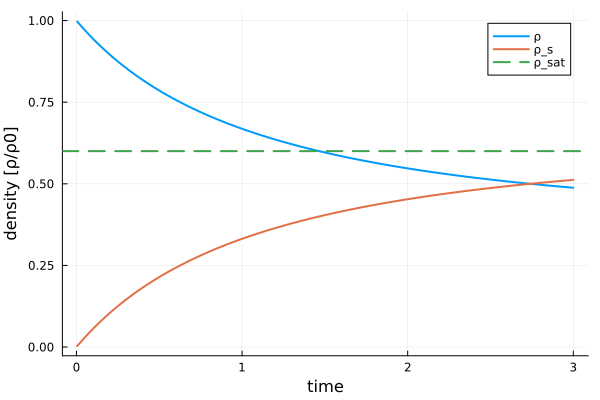
\includegraphics[width=0.6\textwidth]{figures/rho_plot.png}
    \caption{Plot of $\rho$ and $\rho_{sat}$ over time.}\label{fig:model_one_result}
\end{figure}

\subsection*{Model 2}
The results of this model after half a second are shown in Figure~\ref{fig:model_2_results}.

\begin{figure}[h]
    \centering
    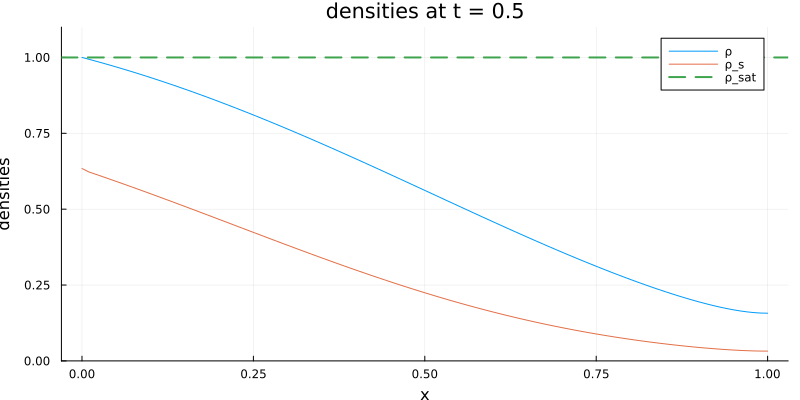
\includegraphics[width=0.8\textwidth]{figures/model_2_result.png}
    \caption{Results at $t=0.5$}\label{fig:model_2_results}
\end{figure}

\subsection*{Model 3}
The results of this model after one second are shown in Figure~\ref{fig:model_3_result}.

\begin{figure}
    \centering
    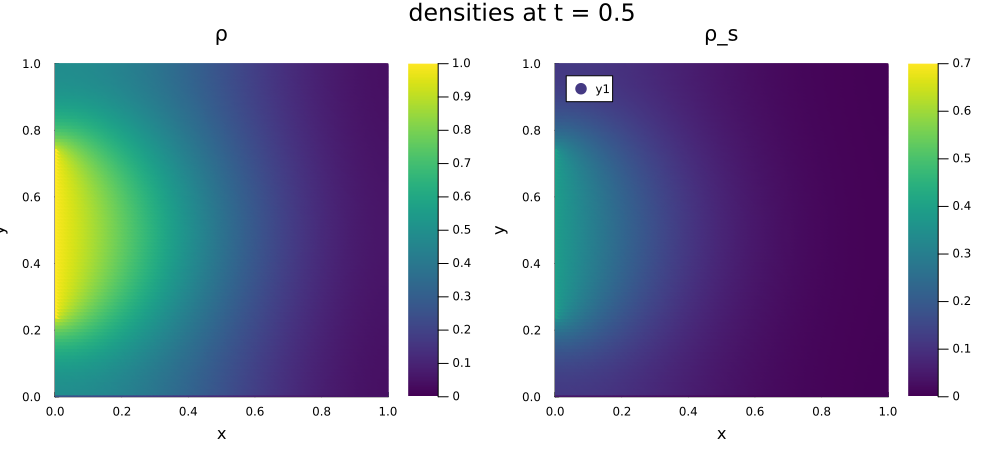
\includegraphics[width=.8\textwidth]{figures/model_3_result.png}
    \caption{Result of model 3 at time $t=1$}\label{fig:model_3_result}
\end{figure}

\subsection*{Model 4}
For the IMEX scheme we have visualized our results in Figure~\ref{fig:model_4_IMEX}, and for the Finite Difference scheme in Figure~\ref{fig:model_4_FD}. The results are similar, but the IMEX scheme is more stable and allows for larger time steps. The Finite Difference scheme requires smaller time steps to maintain stability, which can lead to longer computation times. Overall, the IMEX scheme provides a more efficient and robust solution for this model.

The result for applying total pressure is shown in Figure~\ref{fig:model_4_FD_ptot}. The total pressure is calculated using the formula above, and it shows how the pressure varies along the length of the battery at a specific time. The results indicate that the pressure is highest at the inlet and decreases towards the outlet, which is consistent with the expected behavior of the system.

\begin{figure}
    \centering 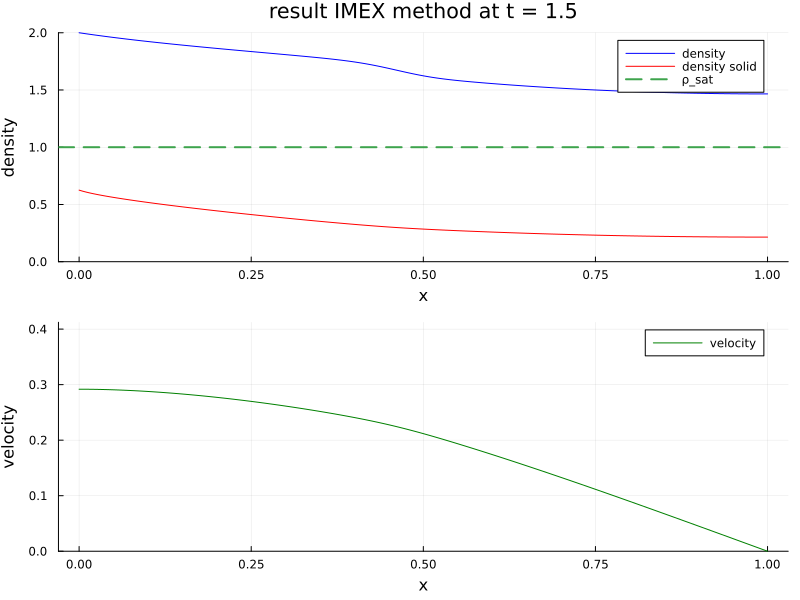
\includegraphics[width=.8\textwidth]{figures/model_4_result_IMEX.png}
    \caption{Results of the IMEX scheme at $t=1.5$.}\label{fig:model_4_IMEX}
\end{figure}

\begin{figure}
    \centering 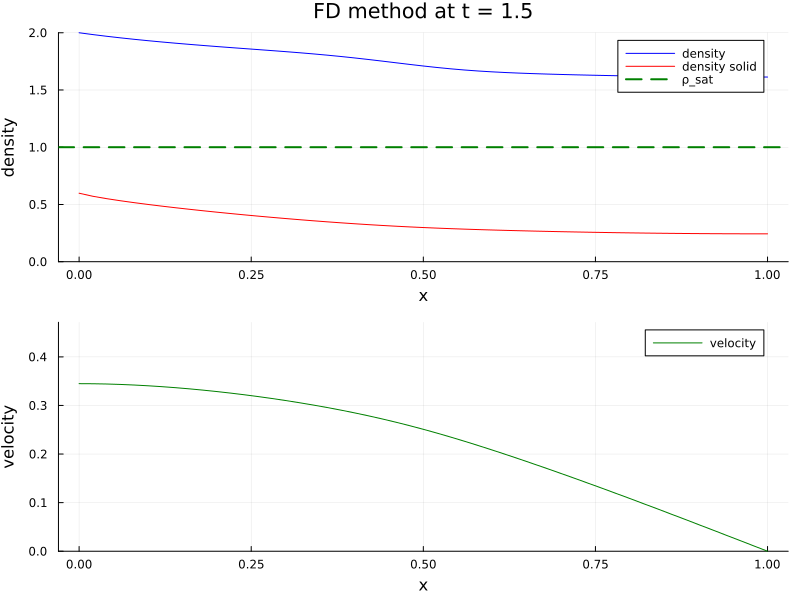
\includegraphics[width=.8\textwidth]{figures/model_4_FD.png}
    \caption{Results of the Finite Difference scheme at $t=1.5$.}\label{fig:model_4_FD}
\end{figure}

\begin{figure}
    \centering 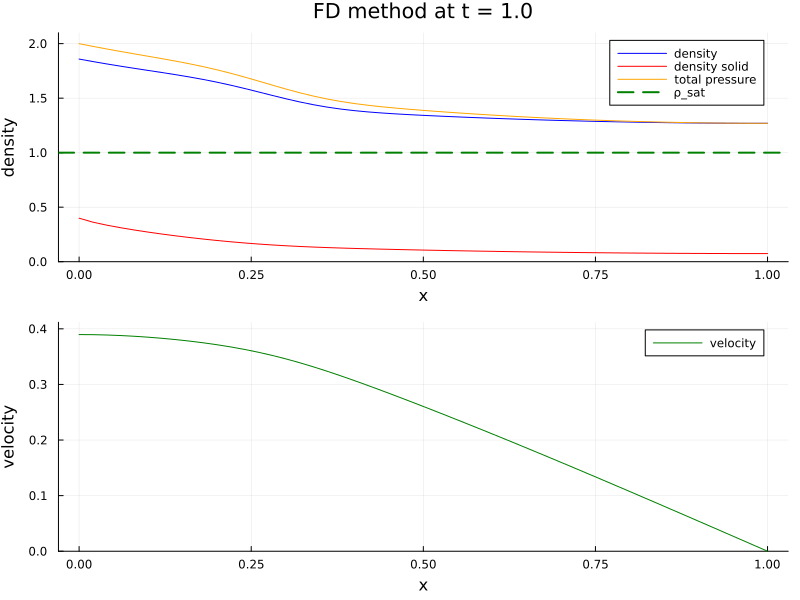
\includegraphics[width=.8\textwidth]{figures/model_4_FD_ptot.png}
    \caption{Results of the Finite Difference scheme with total pressure at $t=1.5$.}\label{fig:model_4_FD_ptot}
\end{figure}

\clearpage
\section{Conclusion}\label{sec:conclusion}
Hier wil ik het ook nog even over hebben!
\setcounter{equation}{0}

% Appendix
\clearpage
\begin{appendices}
\renewcommand{\theequation}{A\arabic{equation}}
\section{Battery integration}
For calculating the absorbed/desorbed amount of energy in a battery, I had to integrate over the domain. I found an easier way to tackle this problem by using the mass matrix and fem indeces already calculated in the spacial discretization. Below is a quick description of this method, which I could not really find a logical place in my thesis for, apart from the appendix.

The amount of absorbed gas stored in the solid phase is obtained by integrating the solid density over the domain:
\begin{equation}
M_s(t)=\int_{\Omega}\rho_s(x,t)\,dx .
\end{equation}
The finite element approximation of the solid density is
\begin{equation}
\rho_s^n(x)=\sum_{i=1}^{N_s} \rho_s^{n,i}\phi_i(x),
\end{equation}
where $N_s$ is the number of solid density degrees of freedom and
$\phi_i$ are the finite element basis functions. Therefore,
\begin{equation}
M_s^n
=
\int_{\Omega}
\sum_{i=1}^{N_s}\rho_s^{n,i}\phi_i(x)\,dx .
\end{equation}
Rearranging the summation gives
\begin{equation}
M_s^n
=
\sum_{i=1}^{N_s}
\rho_s^{n,i}
\int_{\Omega}\phi_i(x)\,dx .
\end{equation}
The integral of each basis function is obtained from the consistent mass matrix.
The mass matrix is defined as
\begin{equation}
(M_s)_{ij}
=
\int_{\Omega}\phi_i(x)\phi_j(x)\,dx .
\end{equation}
Multiplying the mass matrix by a vector of ones gives
\begin{equation}
b_i
=
\sum_{j=1}^{N_s}(M_s)_{ij}
=
\sum_{j=1}^{N_s}
\int_{\Omega}\phi_i(x)\phi_j(x)\,dx .
\end{equation}
Since the finite element basis satisfies the partition of unity,
\begin{equation}
\sum_j\phi_j(x)=1,
\end{equation}
this becomes
\begin{equation}
b_i
=
\int_{\Omega}\phi_i(x)\,dx .
\end{equation}
The total absorbed mass at timestep $n$ is therefore approximated by
\begin{equation}
M_s^n
\approx
\sum_{i=1}^{N_s}b_i\rho_s^{n,i}
=
\mathbf{b}^T\boldsymbol{\rho}_s^n .
\end{equation}  
The maximum possible absorbed mass corresponds to a completely saturated
solid phase:
\begin{equation}
M_{\mathrm{sat}}
=
\int_{\Omega}\rho_{\mathrm{sat}}\,dx
=
\rho_{\mathrm{sat}}|\Omega|,
\end{equation}
where $|\Omega|$ is the domain length (equal to $1$ in the current model).
The filling fraction of the solid storage capacity is then defined as
\begin{equation}
f^n
=
\frac{M_s^n}{M_{\mathrm{sat}}}
=
\frac{\mathbf{b}^T\boldsymbol{\rho}_s^n}
{\rho_{\mathrm{sat}}|\Omega|}.
\end{equation}
A value of
\begin{equation}
f^n=0
\end{equation}
corresponds to an empty solid phase, while
\begin{equation}
f^n=1
\end{equation}
corresponds to a completely saturated solid phase.

\newpage
\end{appendices}



% Bibliography
\clearpage
\nocite{*}
\bibliographystyle{unsrt}
\bibliography{chapters/mybib}

\end{document}